\documentclass[12pt]{article}
\usepackage[utf8]{inputenc}
\usepackage[spanish]{babel}
\usepackage{amsmath, amssymb, geometry, tikz, pgfplots, graphicx} % Se añadió graphicx para las imágenes
\pgfplotsset{compat=1.18}
\geometry{letterpaper, margin=2.5cm}

\begin{document}

% ==========================================
% PORTADA
% ==========================================
\begin{titlepage}
    \centering
    \vspace*{2cm}
    
    {\Large \textbf{UNIVERSIDAD NACIONAL DE COLOMBIA}}\\[0.5cm]
    {\large FACULTAD DE INGENIERÍA}\\[0.5cm]
    {\large DEPARTAMENTO DE INGENIERÍA ELÉCTRICA Y ELECTRÓNICA}\\[0.5cm]
    {\large SEÑALES Y SISTEMAS I}\\[2cm]
    
    {\Huge \textbf{Taller 2 y Laboratorio 1}}\\[0.5cm]
    {\Large \textbf{Propiedades de las Señales}}\\[3cm]
    
    {\large \textbf{Integrantes:}}\\[0.5cm]
    {\large Juan José Tobar Álvarez - jutobara@unal.edu.co}\\[0.2cm]
    {\large Nombre del Integrante 2 - Código}\\[0.2cm]
    {\large Nombre del Integrante 3 - Código}\\[3cm]
    
    \vfill
    {\large \today}\\[1cm]
\end{titlepage}

% ==========================================
% DESARROLLO DEL TALLER
% ==========================================
\section*{1. Taller 2: Propiedades de las señales}

\subsection*{1. Componentes par e impar de las señales}
Por definición, la parte par $x_p(t)$ y la parte impar $x_i(t)$ de una señal continua $x(t)$ se determinan mediante:
\begin{equation*}
    x_p(t) = \frac{x(t) + x(-t)}{2}, \quad x_i(t) = \frac{x(t) - x(-t)}{2}
\end{equation*}

\textbf{a) $x(t) = \cos(t) + \sin(t) + \sin(t)\cos(t)$}
Evaluamos $x(-t)$ teniendo en cuenta que $\cos(-t) = \cos(t)$ (función par) y $\sin(-t) = -\sin(t)$ (función impar):
\begin{align*}
    x(-t) &= \cos(-t) + \sin(-t) + \sin(-t)\cos(-t) \\
          &= \cos(t) - \sin(t) - \sin(t)\cos(t)
\end{align*}
Hallamos $x_p(t)$ y $x_i(t)$:
\begin{align*}
    x_p(t) &= \frac{[\cos(t) + \sin(t) + \sin(t)\cos(t)] + [\cos(t) - \sin(t) - \sin(t)\cos(t)]}{2} = \cos(t) \\
    x_i(t) &= \frac{[\cos(t) + \sin(t) + \sin(t)\cos(t)] - [\cos(t) - \sin(t) - \sin(t)\cos(t)]}{2} = \sin(t) + \sin(t)\cos(t)
\end{align*}

\textbf{b) $x(t) = 1 + t\cos(t) + t^2\sin(t) + t^3\sin(t)\cos(t)$}
Evaluamos $x(-t)$:
\begin{align*}
    x(-t) &= 1 + (-t)\cos(-t) + (-t)^2\sin(-t) + (-t)^3\sin(-t)\cos(-t) \\
          &= 1 - t\cos(t) - t^2\sin(t) + t^3\sin(t)\cos(t)
\end{align*}
Componentes:
\begin{align*}
    x_p(t) &= \frac{x(t) + x(-t)}{2} = 1 + t^3\sin(t)\cos(t) \\
    x_i(t) &= \frac{x(t) - x(-t)}{2} = t\cos(t) + t^2\sin(t)
\end{align*}

\textbf{c) $x(t) = (1 + t^3)\cos^3(10t) = \cos^3(10t) + t^3\cos^3(10t)$}
Evaluamos $x(-t)$:
\begin{align*}
    x(-t) &= (1 + (-t)^3)\cos^3(-10t) = (1 - t^3)\cos^3(10t) = \cos^3(10t) - t^3\cos^3(10t)
\end{align*}
Componentes:
\begin{align*}
    x_p(t) &= \frac{x(t) + x(-t)}{2} = \cos^3(10t) \\
    x_i(t) &= \frac{x(t) - x(-t)}{2} = t^3\cos^3(10t)
\end{align*}

% ---------------------------------------------------
\subsection*{2. Clasificación de energía o potencia}

\textbf{a) Señal continua $x(t)$}
\begin{equation*}
x(t) = \begin{cases} t, & 0 \le t \le 1 \\ 2-t, & 1 < t \le 2 \\ 0, & \text{en otro caso} \end{cases}
\end{equation*}
Como es una señal de duración finita, es una \textbf{señal de energía}. Su potencia promedio es cero ($P = 0$).
\begin{align*}
    E &= \int_{-\infty}^{\infty} |x(t)|^2 dt = \int_{0}^{1} t^2 dt + \int_{1}^{2} (2-t)^2 dt \\
      &= \left[ \frac{t^3}{3} \right]_0^1 + \left[ -\frac{(2-t)^3}{3} \right]_1^2 = \frac{1}{3} + \left(0 - \left(-\frac{1}{3}\right)\right) = \frac{2}{3} \text{ Joules}
\end{align*}

\textbf{b) Señal discreta $x[n]$}
\begin{equation*}
x[n] = \begin{cases} \cos(\pi n), & n \ge 0 \\ 0, & n < 0 \end{cases}
\end{equation*}
La señal no se anula al tender al infinito (toma valores $1, -1, 1, -1 \dots$), por lo que tiene energía infinita. Es una \textbf{señal de potencia}.
\begin{align*}
    P &= \lim_{N \to \infty} \frac{1}{2N+1} \sum_{n=-N}^{N} |x[n]|^2 = \lim_{N \to \infty} \frac{1}{2N+1} \sum_{n=0}^{N} |\cos(\pi n)|^2 \\
      &= \lim_{N \to \infty} \frac{1}{2N+1} \sum_{n=0}^{N} 1 = \lim_{N \to \infty} \frac{N+1}{2N+1} = \frac{1}{2} \text{ Watts}
\end{align*}

\textbf{c) Señal discreta $x[n]$}
\begin{equation*}
x[n] = \begin{cases} n, & 0 \le n \le 5 \\ 10-n, & 5 < n \le 10 \\ 0, & \text{en otro caso} \end{cases}
\end{equation*}
Es una señal de duración finita discreta, por lo tanto es una \textbf{señal de energía} ($P = 0$).
\begin{align*}
    E &= \sum_{n=-\infty}^{\infty} |x[n]|^2 = \sum_{n=0}^{5} n^2 + \sum_{n=6}^{10} (10-n)^2 \\
      &= (0^2 + 1^2 + 2^2 + 3^2 + 4^2 + 5^2) + (4^2 + 3^2 + 2^2 + 1^2 + 0^2) \\
      &= (0 + 1 + 4 + 9 + 16 + 25) + (16 + 9 + 4 + 1 + 0) = 55 + 30 = 85 \text{ Joules}
\end{align*}

% ---------------------------------------------------
\subsection*{3. Sistema no lineal: Salida cuadrática}
Dada la señal de entrada $x(t) = 3\cos\left(200t + \frac{\pi}{6}\right)$ y la relación de salida $y(t) = x^2(t)$:
\begin{equation*}
    y(t) = \left[ 3\cos\left(200t + \frac{\pi}{6}\right) \right]^2 = 9\cos^2\left(200t + \frac{\pi}{6}\right)
\end{equation*}
Aplicando la identidad trigonométrica provista $\cos^2(\theta) = \frac{1}{2}[1 + \cos(2\theta)]$:
\begin{align*}
    y(t) &= 9 \left( \frac{1}{2} \left[ 1 + \cos\left(2\left(200t + \frac{\pi}{6}\right)\right) \right] \right) \\
         &= \frac{9}{2} + \frac{9}{2}\cos\left(400t + \frac{\pi}{3}\right)
\end{align*}
De esta expresión deducimos:
\begin{itemize}
    \item \textbf{Componente DC:} $\frac{9}{2} = 4.5$
    \item \textbf{Componente sinusoidal:} 
    \begin{itemize}
        \item Amplitud: $\frac{9}{2} = 4.5$
        \item Frecuencia fundamental ($\omega_0$): $400 \text{ rad/s}$
    \end{itemize}
\end{itemize}

% ---------------------------------------------------
\subsection*{4. Energía del pulso cosenoidal}
Señal definida como $x(t) = \frac{1}{2}(\cos(\omega t) + 1)$ para $t \in \left[-\frac{\pi}{\omega}, \frac{\pi}{\omega}\right]$.
\begin{align*}
    E &= \int_{-\pi/\omega}^{\pi/\omega} \left[ \frac{1}{2}(\cos(\omega t) + 1) \right]^2 dt = \frac{1}{4} \int_{-\pi/\omega}^{\pi/\omega} (\cos^2(\omega t) + 2\cos(\omega t) + 1) dt \\
      &= \frac{1}{4} \int_{-\pi/\omega}^{\pi/\omega} \left( \frac{1 + \cos(2\omega t)}{2} + 2\cos(\omega t) + 1 \right) dt \\
      &= \frac{1}{4} \int_{-\pi/\omega}^{\pi/\omega} \left( \frac{3}{2} + 2\cos(\omega t) + \frac{1}{2}\cos(2\omega t) \right) dt \\
      &= \frac{1}{4} \left[ \frac{3}{2}t + \frac{2}{\omega}\sin(\omega t) + \frac{1}{4\omega}\sin(2\omega t) \right]_{-\pi/\omega}^{\pi/\omega}
\end{align*}
Al evaluar los límites, las funciones seno se anulan en múltiplos de $\pi$:
\begin{equation*}
    E = \frac{1}{4} \left( \frac{3}{2}\left(\frac{\pi}{\omega}\right) - \frac{3}{2}\left(-\frac{\pi}{\omega}\right) \right) = \frac{1}{4} \left( \frac{3\pi}{\omega} \right) = \frac{3\pi}{4\omega} \text{ Joules}
\end{equation*}

% ---------------------------------------------------
\subsection*{5. Energía del pulso trapezoidal}
El pulso está dado en tramos entre $-5$ y $5$.
\begin{align*}
    E &= \int_{-5}^{-4} (t+5)^2 dt + \int_{-4}^{4} (1)^2 dt + \int_{4}^{5} (5-t)^2 dt \\
      &= \left[ \frac{(t+5)^3}{3} \right]_{-5}^{-4} + \left[ t \right]_{-4}^{4} + \left[ -\frac{(5-t)^3}{3} \right]_{4}^{5} \\
      &= \left(\frac{1}{3} - 0\right) + (4 - (-4)) + \left(0 - \left(-\frac{1}{3}\right)\right) \\
      &= \frac{1}{3} + 8 + \frac{1}{3} = \frac{26}{3} \text{ Joules}
\end{align*}

% ---------------------------------------------------
\subsection*{6. Demostración de energía por paridad}
Partimos de la descomposición de la señal $x(t) = x_p(t) + x_i(t)$ y elevamos al cuadrado:
\begin{align*}
    E &= \int_{-\infty}^{\infty} [x_p(t) + x_i(t)]^2 dt \\
      &= \int_{-\infty}^{\infty} [x_p^2(t) + x_i^2(t) + 2x_p(t)x_i(t)] dt \\
      &= \int_{-\infty}^{\infty} x_p^2(t) dt + \int_{-\infty}^{\infty} x_i^2(t) dt + 2\int_{-\infty}^{\infty} x_p(t)x_i(t) dt
\end{align*}
El término cruzado es el producto de una función par y una función impar, lo que da como resultado una función impar. La integral de una función impar en un intervalo simétrico ($-\infty$ a $\infty$) es estrictamente cero:
\begin{equation*}
    2\int_{-\infty}^{\infty} \underbrace{x_p(t)x_i(t)}_{\text{Impar}} dt = 0
\end{equation*}
Por lo tanto, se demuestra que:
\begin{equation*}
    E = \int_{-\infty}^{\infty} x_p^2(t) dt + \int_{-\infty}^{\infty} x_i^2(t) dt
\end{equation*}

% ---------------------------------------------------
\newpage
\subsection*{7. Transformaciones del pulso triangular}

La señal original $x(t)$ se define por partes como un pulso triangular con base en $[-1, 1]$ y pico en el origen:
\begin{equation*}
x(t) = \begin{cases} 
t+1, & -1 \le t \le 0 \\ 
-t+1, & 0 < t \le 1 \\ 
0, & \text{en otro caso} 
\end{cases}
\end{equation*}

\textbf{a) Señal $x(-2t-1)$:}
Para hallar el nuevo intervalo activo, igualamos el argumento de la función a los límites originales:
\begin{equation*}
-1 \le -2t-1 \le 1 \implies 0 \le -2t \le 2 \implies -1 \le t \le 0
\end{equation*}
El pico ocurre cuando el argumento es cero ($-2t-1 = 0 \implies t = -0.5$). Es decir, la señal sufre un desplazamiento hacia la izquierda, compresión por un factor de 2 y reflexión en el tiempo.

\begin{figure}[h!]
    \centering
    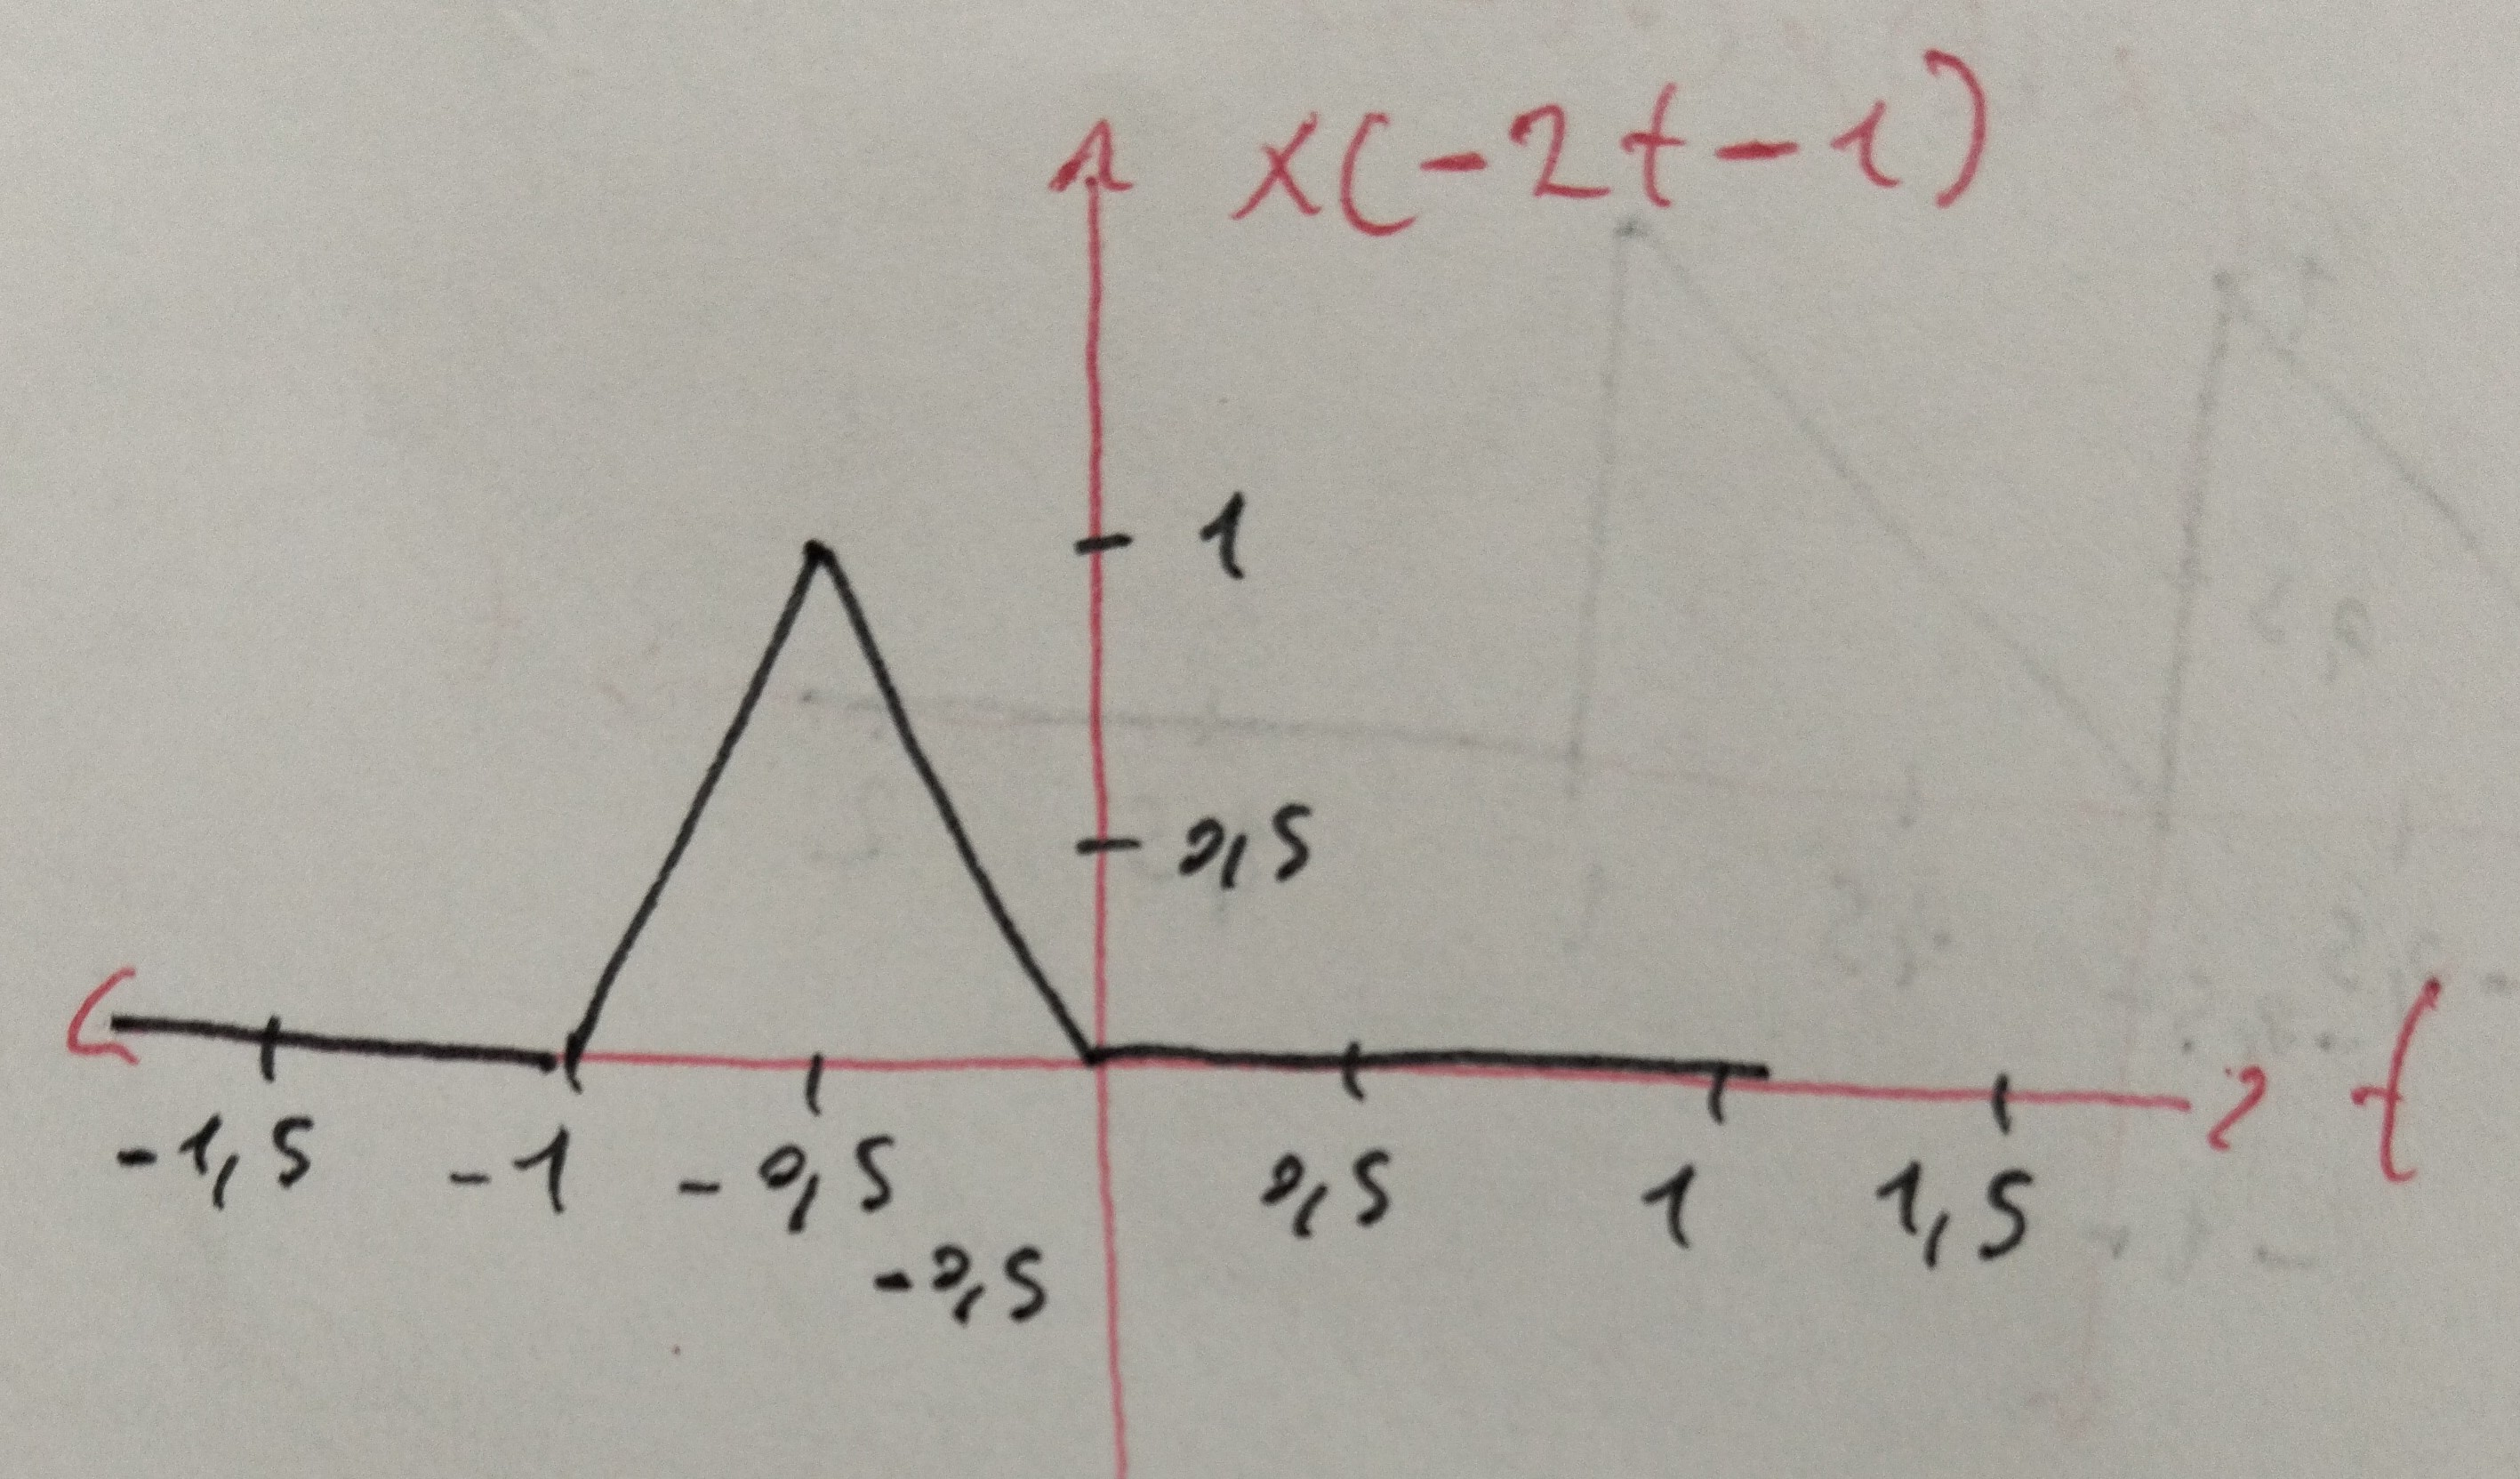
\includegraphics[width=0.6\textwidth]{Punto7Fig1.jpg}
    \caption{Señal $x(-2t-1)$}
\end{figure}

\textbf{b) Señal $x(2(t+2)) = x(2t+4)$:}
Determinamos el intervalo activo evaluando el argumento:
\begin{equation*}
-1 \le 2t+4 \le 1 \implies -5 \le 2t \le -3 \implies -2.5 \le t \le -1.5
\end{equation*}
El pico se ubica en $2t+4 = 0 \implies t = -2$. La señal fue desplazada a la izquierda y comprimida.

\begin{figure}[h!]
    \centering
    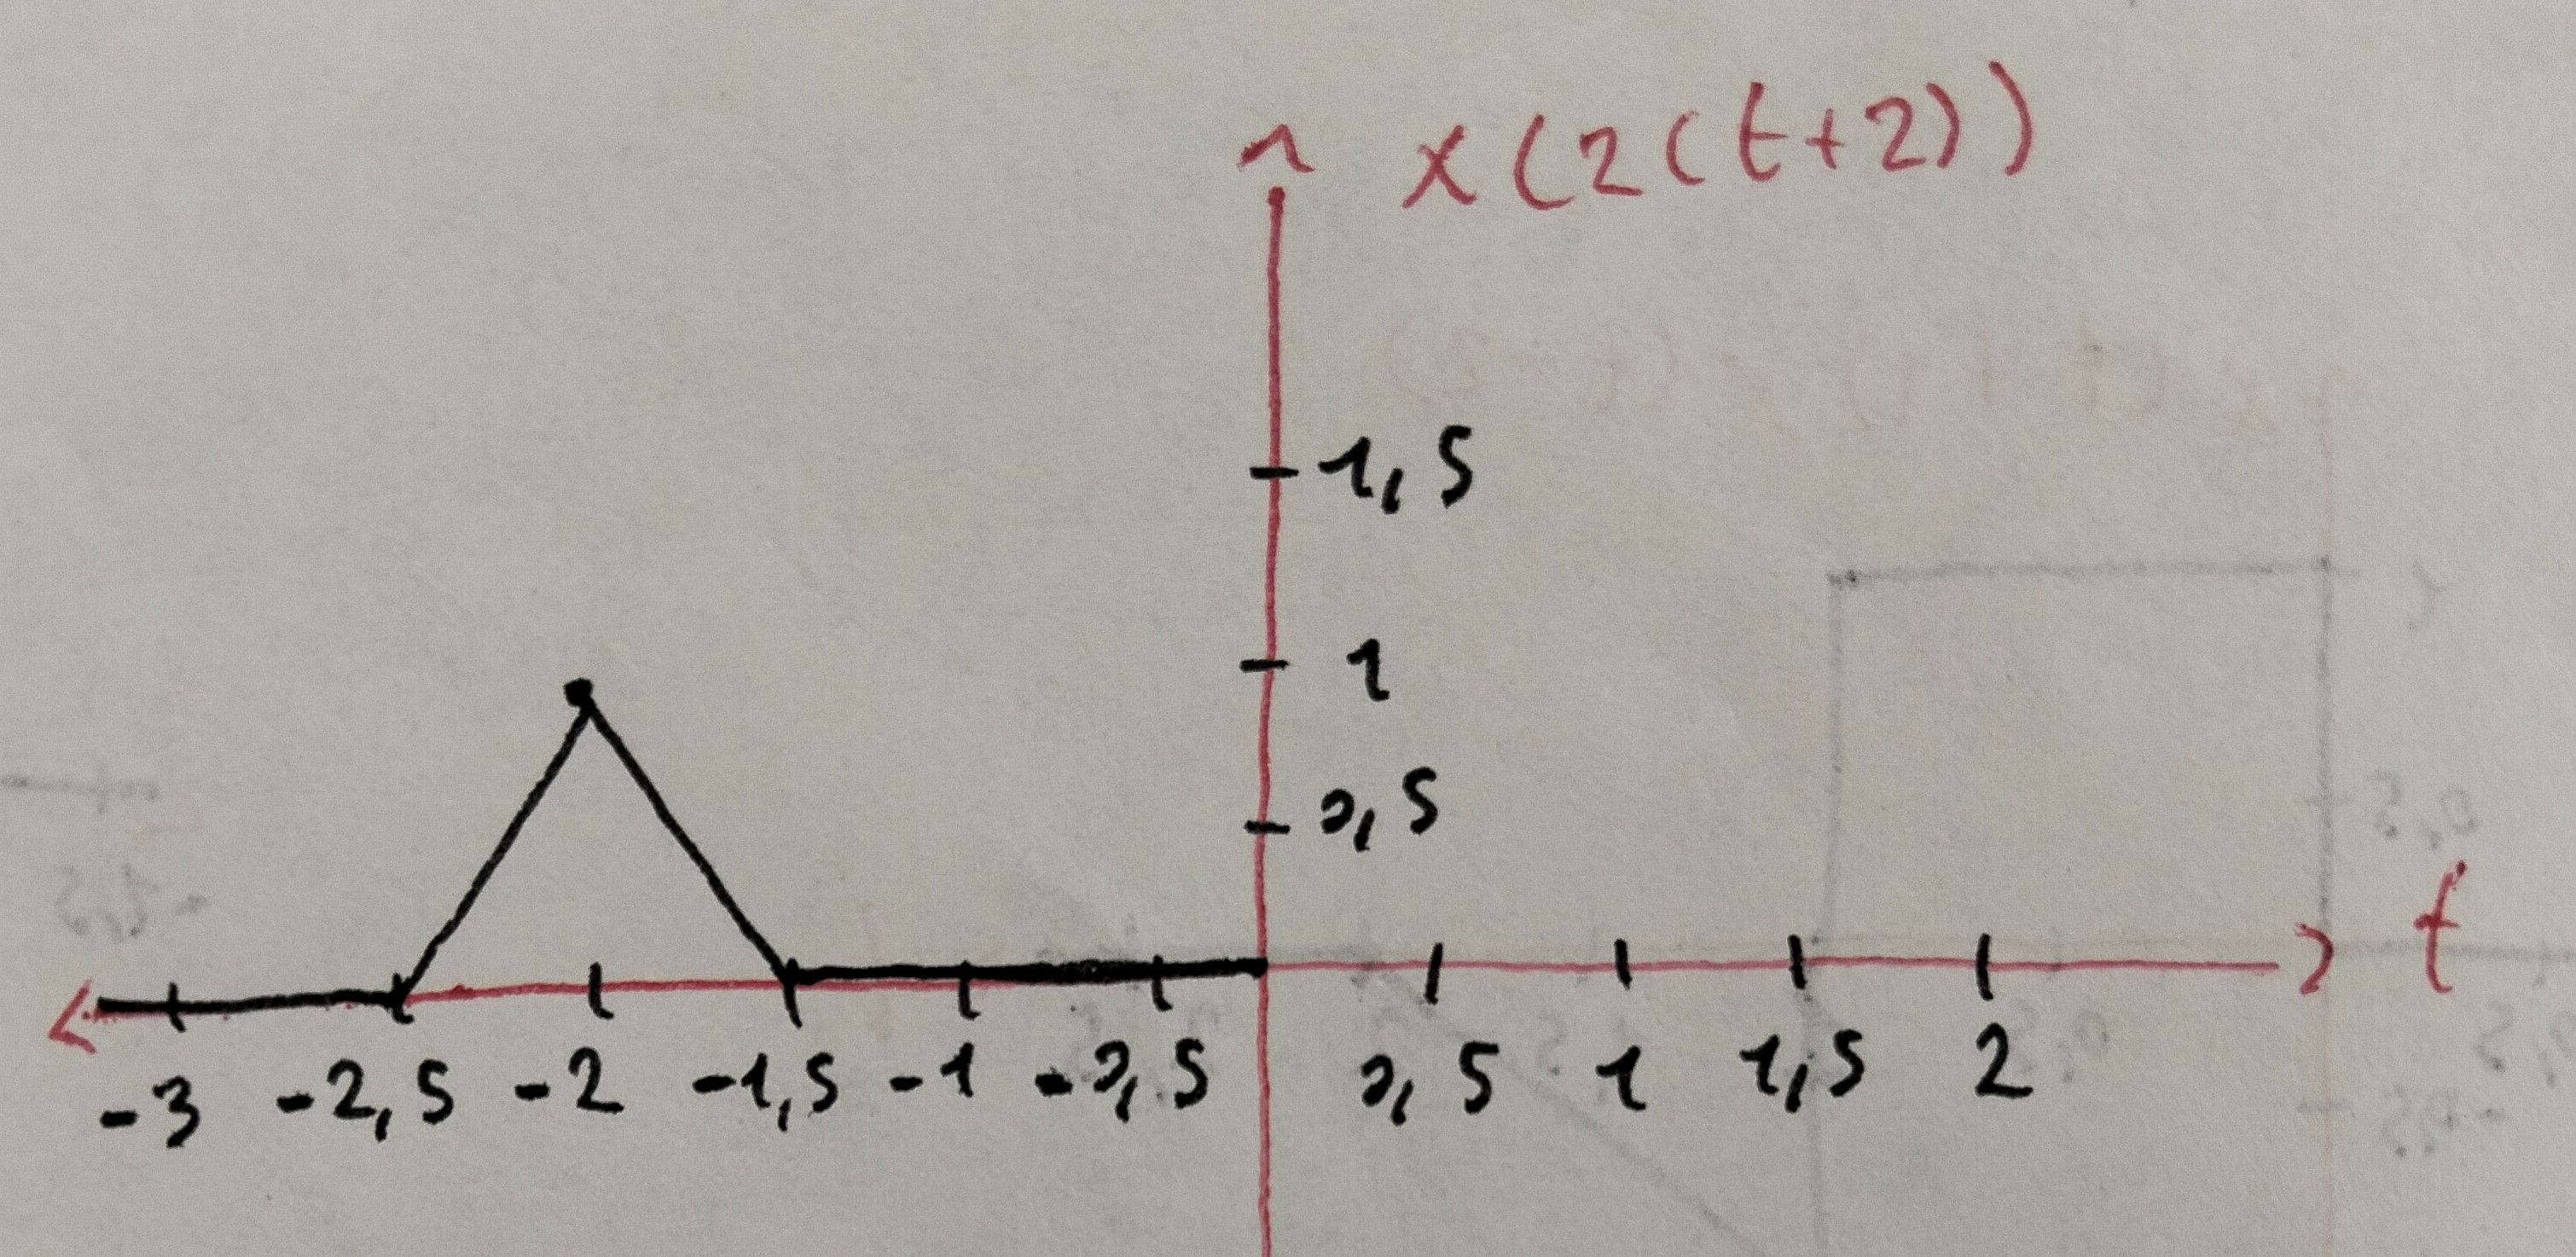
\includegraphics[width=0.6\textwidth]{Punto7Fig2.jpg}
    \caption{Señal $x(2(t+2))$}
\end{figure}

\textbf{c) Señal $x(3t) + x(3t+2)$:}
Analizamos cada término por separado:
\begin{itemize}
    \item $x(3t)$ es activa si $-1 \le 3t \le 1 \implies t \in [-1/3, 1/3]$, con su pico en $t=0$.
    \item $x(3t+2)$ es activa si $-1 \le 3t+2 \le 1 \implies -3 \le 3t \le -1 \implies t \in [-1, -1/3]$, con pico en $t=-2/3$.
\end{itemize}
Ambos pulsos se tocan exactamente en $t = -1/3$ (donde ambos valen 0). La señal resultante consta de dos picos distintos.

\begin{figure}[h!]
    \centering
    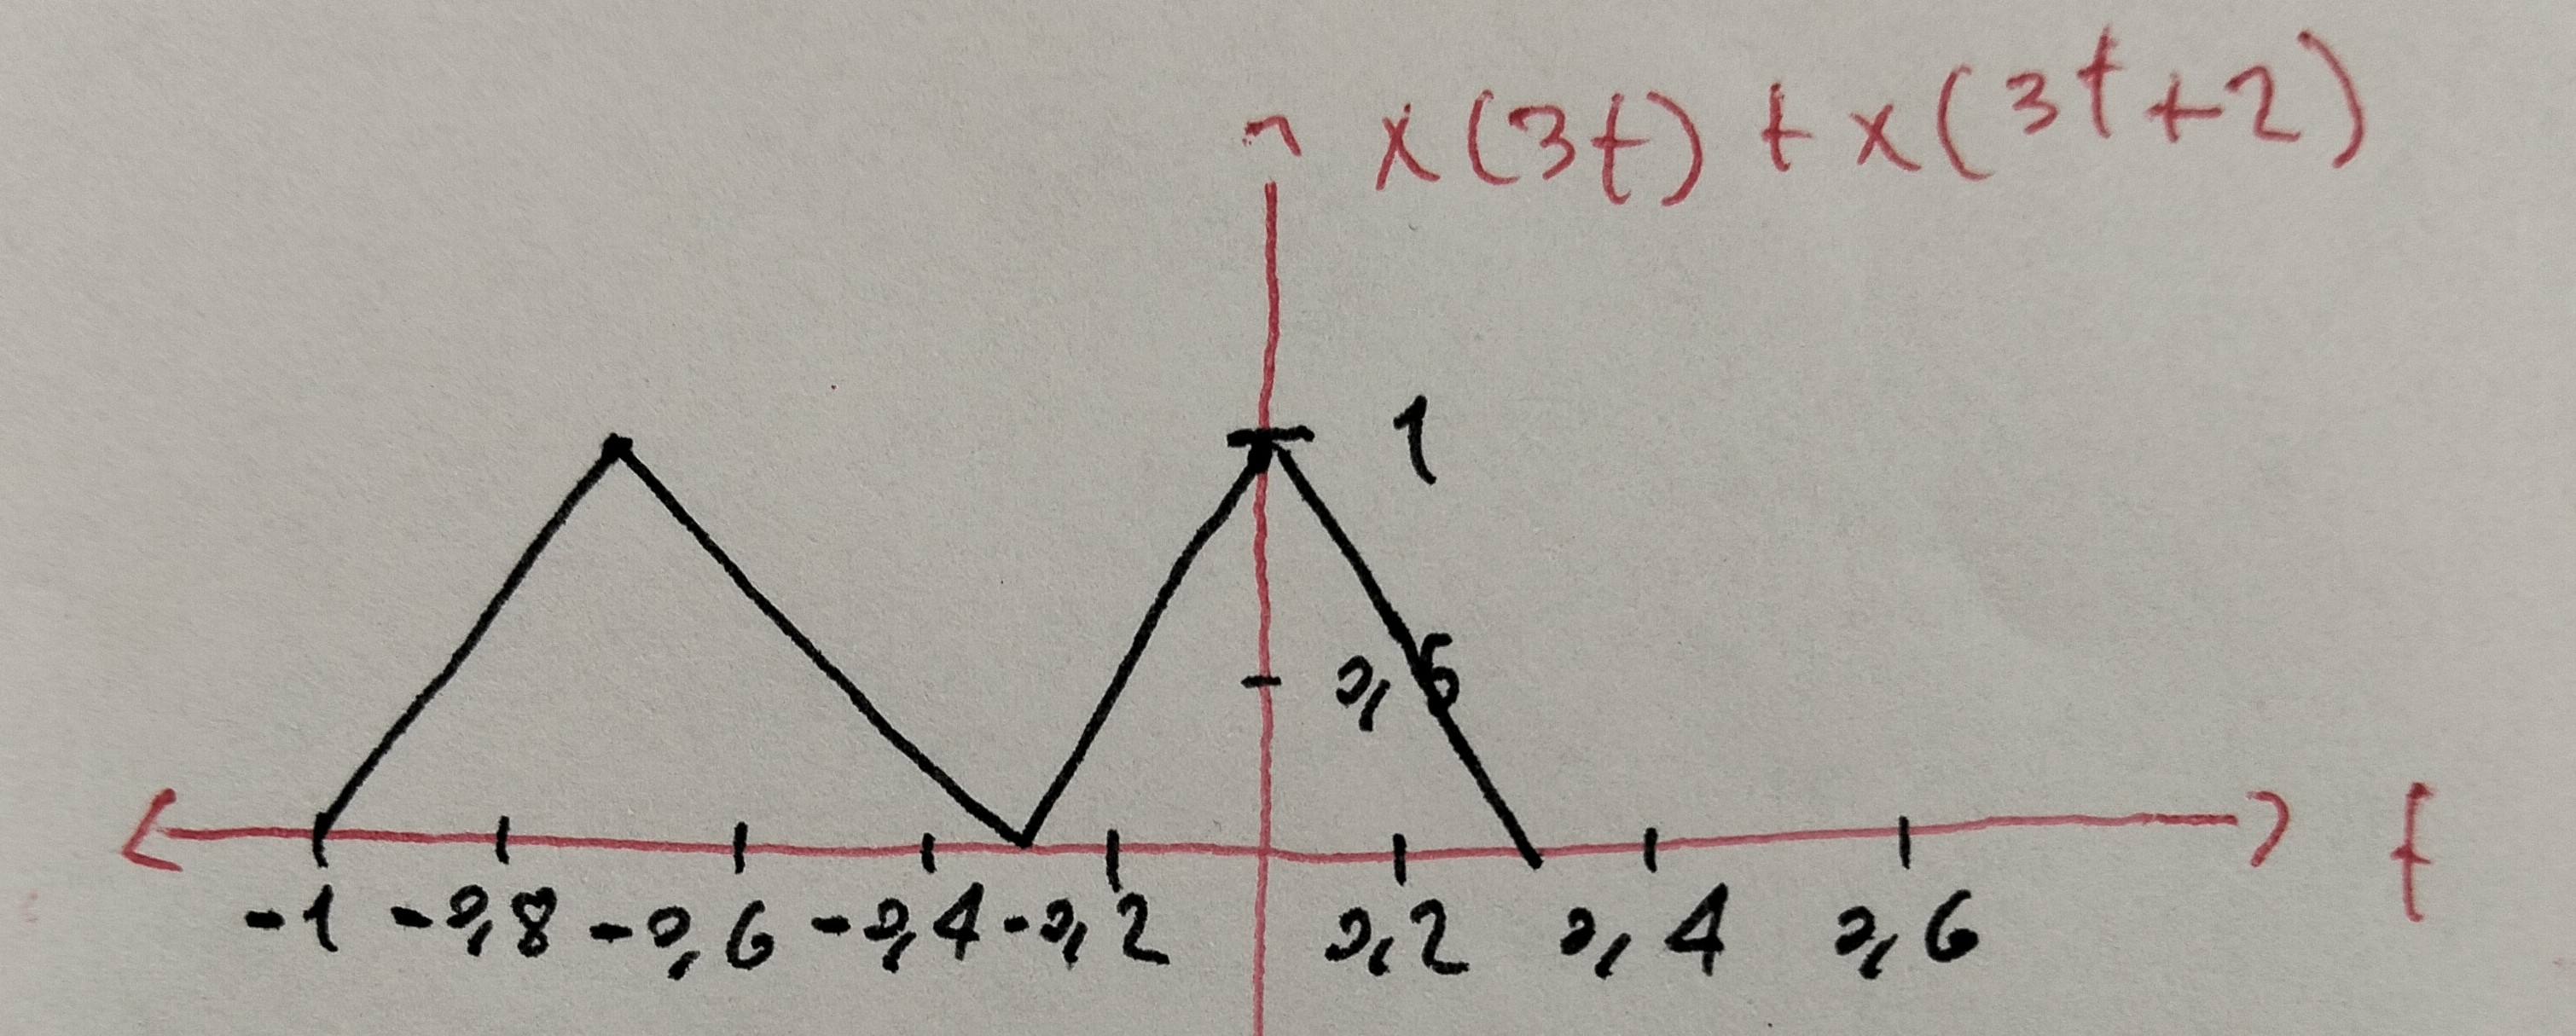
\includegraphics[width=0.6\textwidth]{Punto7Fig3.jpg}
    \caption{Señal $x(3t) + x(3t+2)$}
\end{figure}

% ---------------------------------------------------
\newpage
\subsection*{8. Multiplicación de señales $x(t)$ y $y(t)$}

A partir de las gráficas proporcionadas en el enunciado, establecemos las ecuaciones de cada señal por tramos:
\begin{equation*}
x(t) = \begin{cases} 
-t-1, & -1 \le t < 0 \\ 
t, & 0 \le t < 1 \\ 
1, & 1 \le t < 2 \\ 
3-t, & 2 \le t \le 3 \\ 
0, & \text{resto} 
\end{cases}
\quad\quad
y(t) = \begin{cases} 
1, & -2 \le t < -1 \\ 
-1, & -1 \le t < 0 \\ 
t-1, & 0 \le t < 1 \\ 
1, & 1 \le t \le 2 \\ 
0, & \text{resto} 
\end{cases}
\end{equation*}

\textbf{a) Señal $x(t)y(t-1)$}\\
La señal $y(t-1)$ está desplazada 1 unidad hacia la derecha, por lo que su rango activo cambia a $t \in [-1, 3]$. Se intersecta con $x(t)$ en el mismo intervalo $[-1, 3]$. Multiplicando por tramos:
\begin{itemize}
    \item $t \in [-1, 0)$: $x(t)(-1-1) \to (-t-1)(1) = -t-1$
    \item $t \in [0, 1)$: $x(t)(-1) \to (t)(-1) = -t$
    \item $t \in [1, 2)$: $x(t)(t-2) \to (1)(t-2) = t-2$
    \item $t \in [2, 3]$: $x(t)(1) \to (3-t)(1) = 3-t$
\end{itemize}

\begin{figure}[h!]
    \centering
    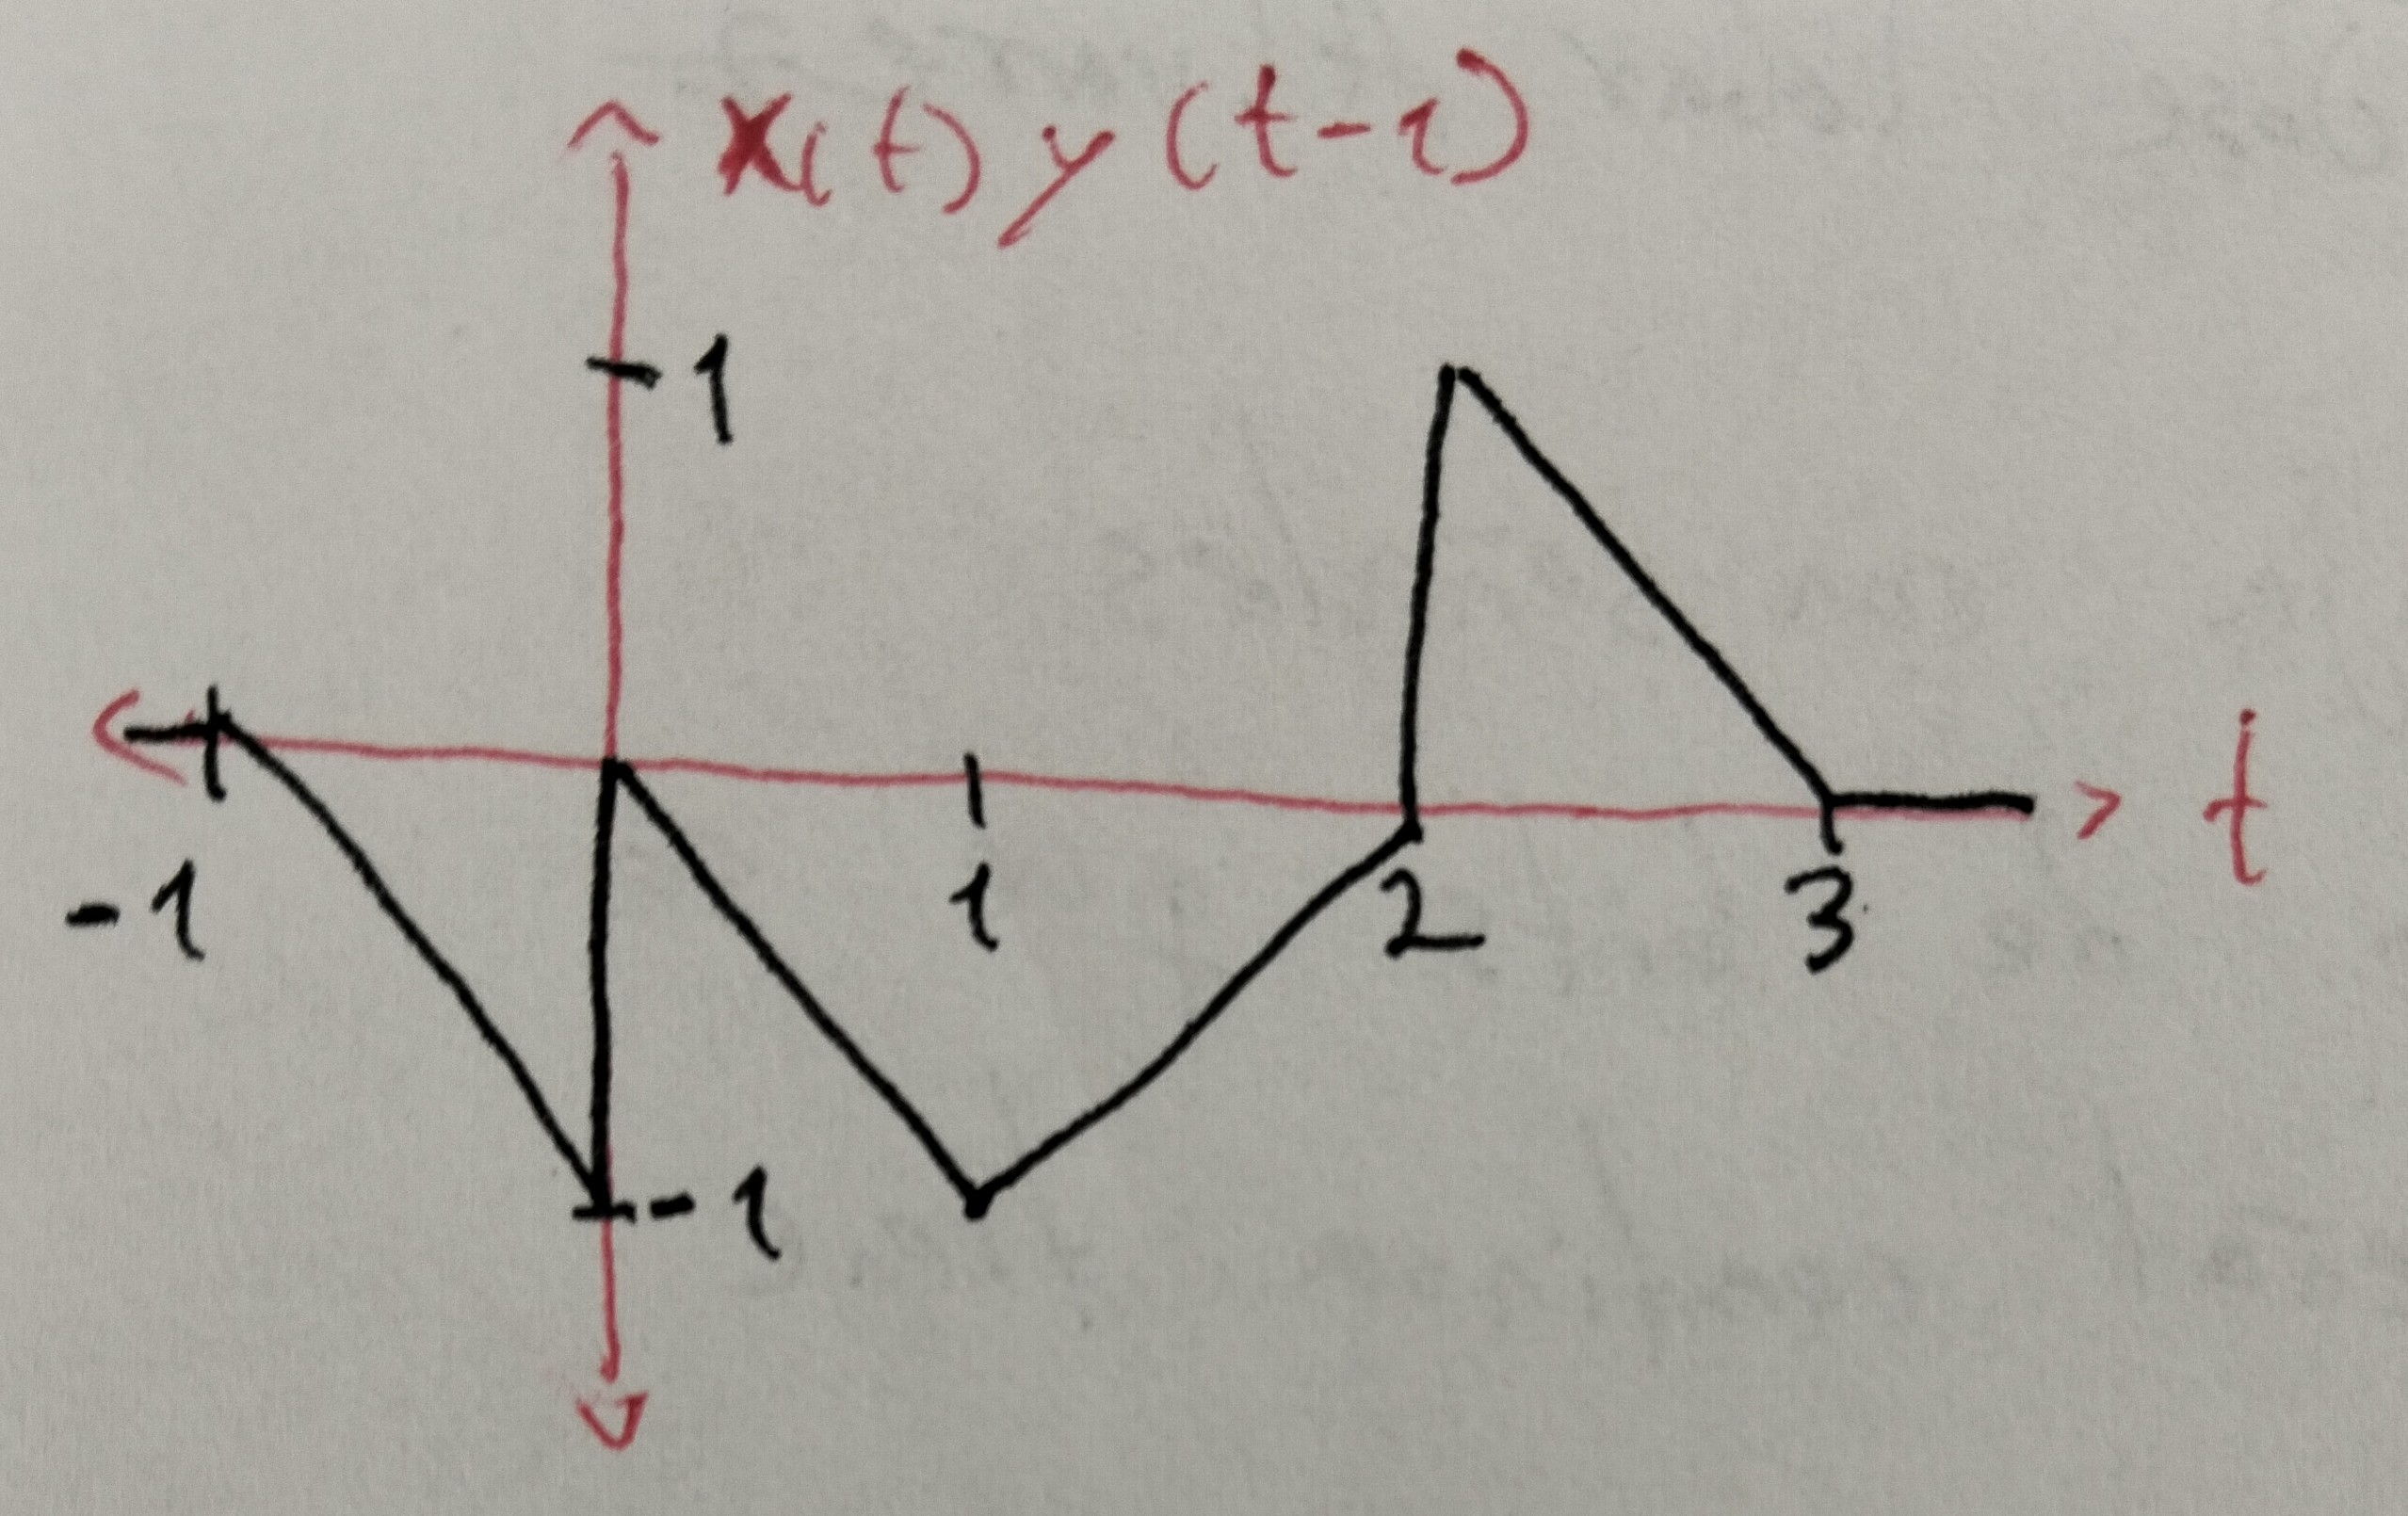
\includegraphics[width=0.6\textwidth]{Punto8Fig1.jpg}
    \caption{Señal $x(t)y(t-1)$}
\end{figure}

\textbf{b) Señal $x(t-1)y(-t)$}\\
La señal $x(t-1)$ está desplazada a la derecha, activa en $[0, 4]$. La señal $y(-t)$ está reflejada, activa en $[-2, 2]$. El traslape de ambas es el intervalo $t \in [0, 2]$:
\begin{itemize}
    \item $t \in [0, 1)$: $x(t-1) = -t$ y $y(-t) = -1$. El producto es $(-t)(-1) = t$.
    \item $t \in [1, 2]$: $x(t-1) = t-1$ y $y(-t) = 1$. El producto es $(t-1)(1) = t-1$.
\end{itemize}
En $t=1$, la señal presenta una discontinuidad pasando de $1$ a $0$.

\begin{figure}[h!]
    \centering
    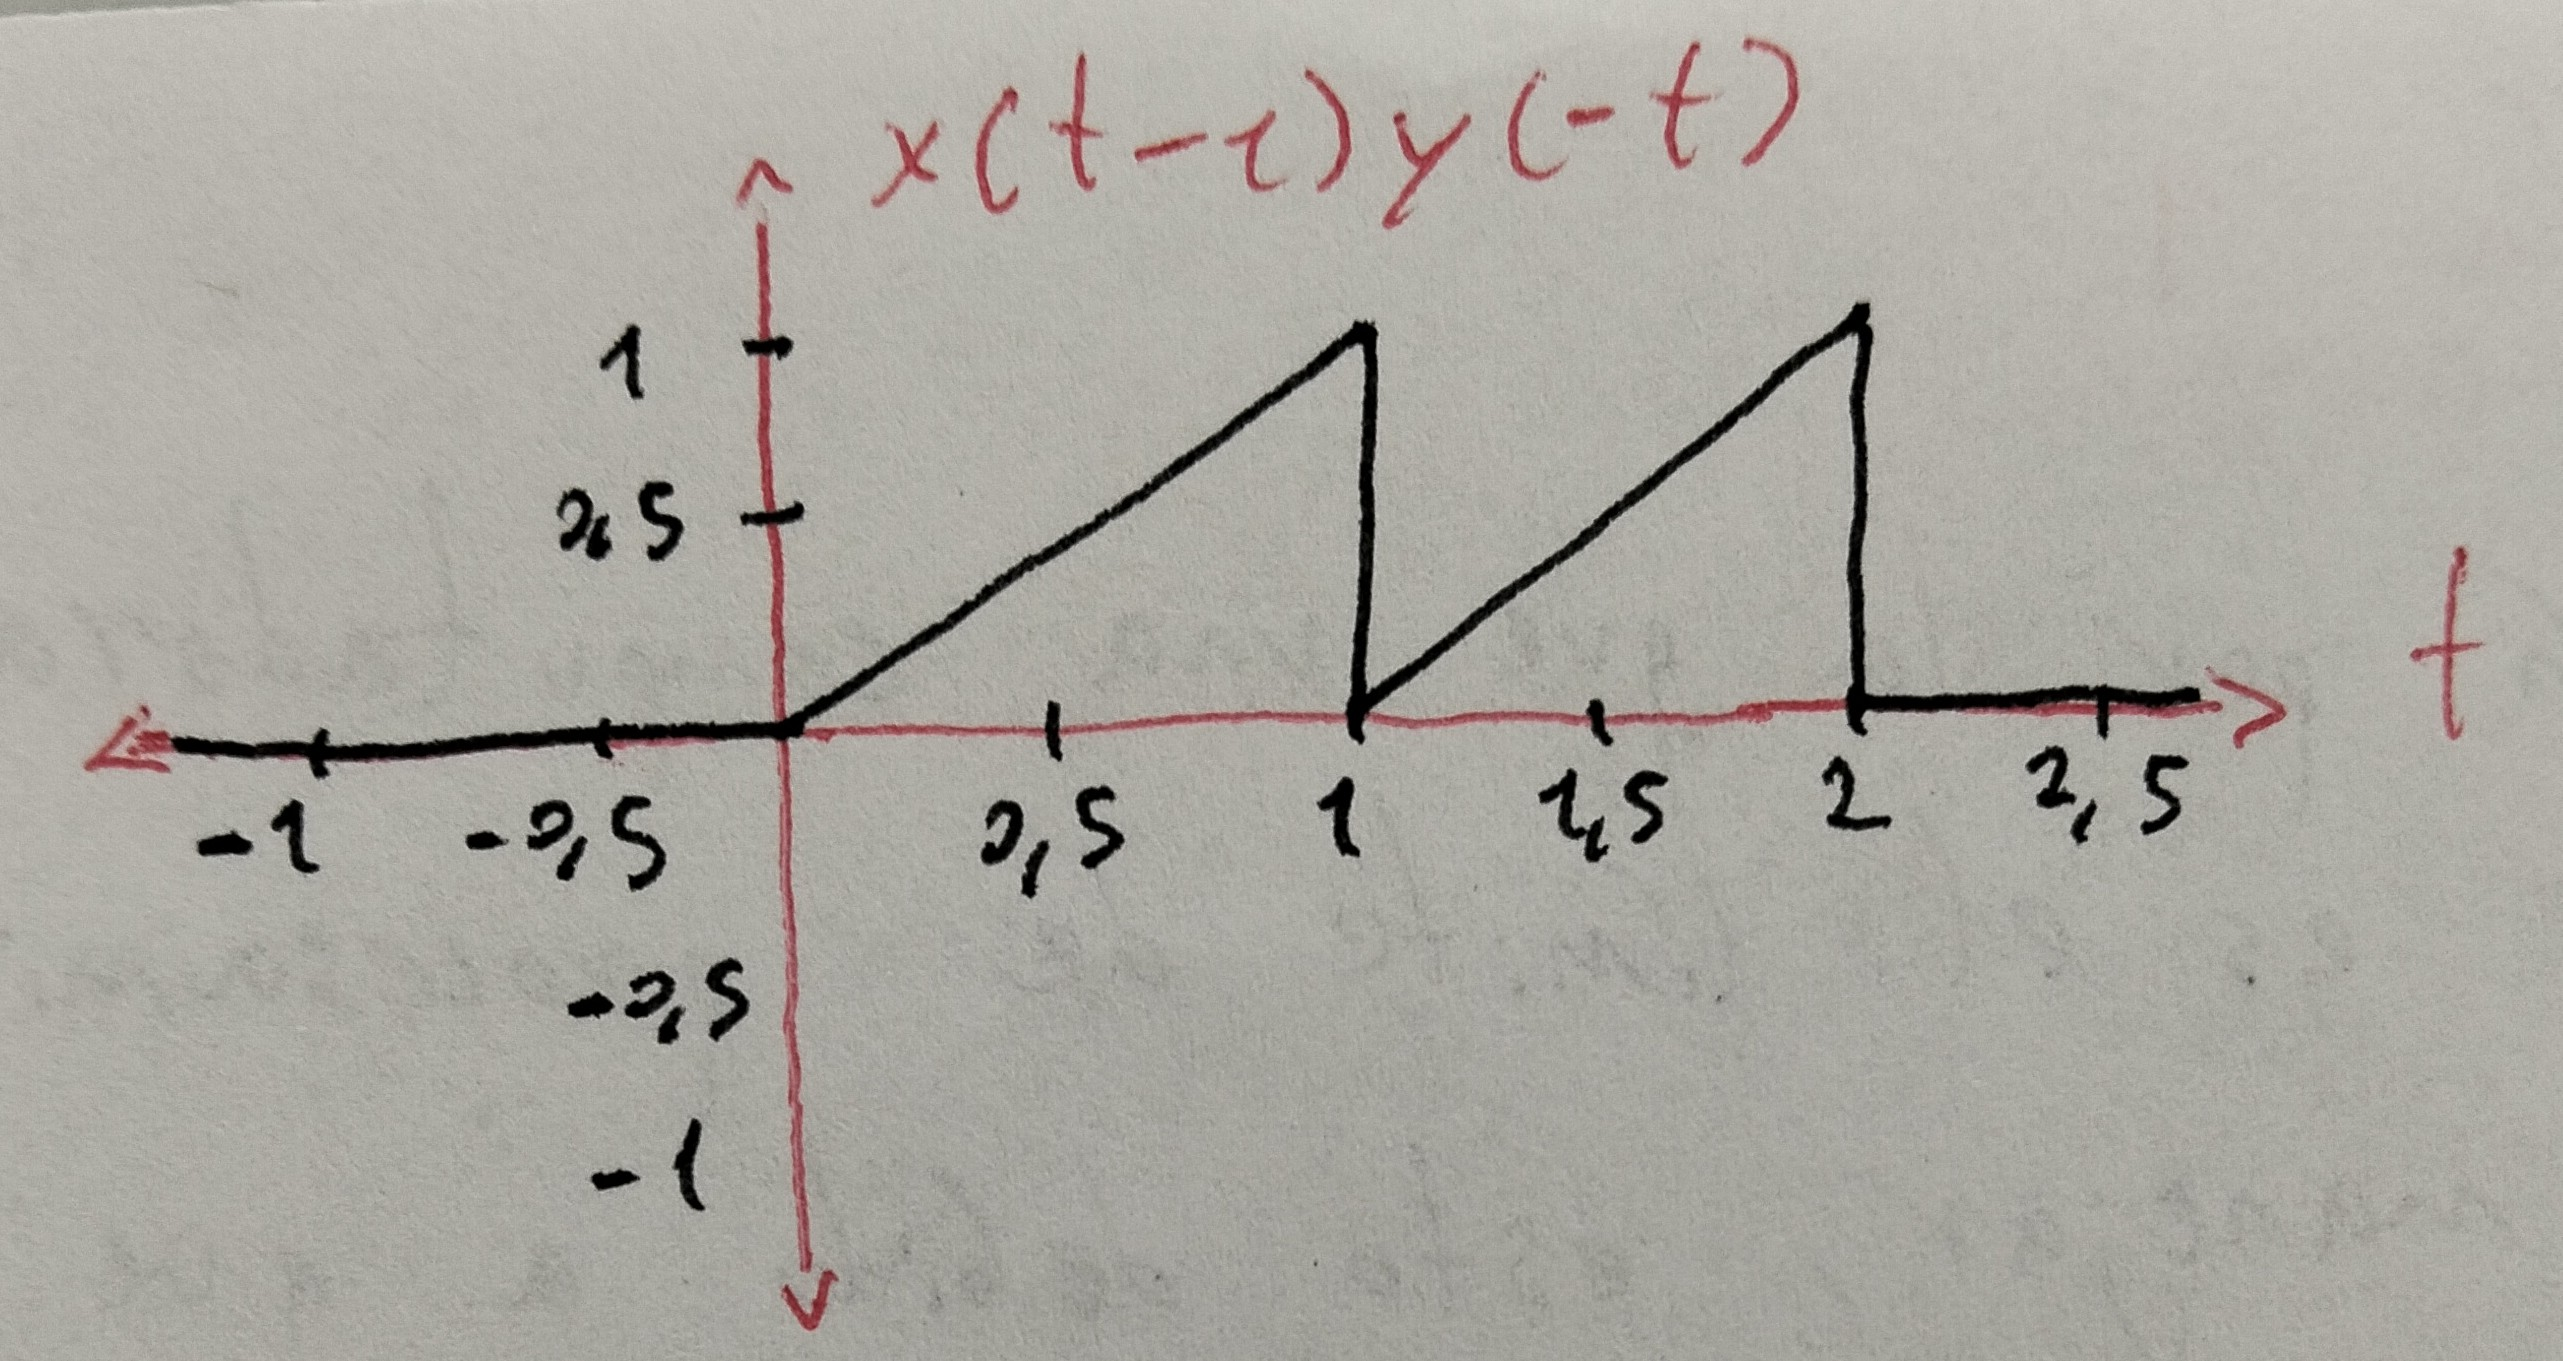
\includegraphics[width=0.6\textwidth]{Punto8Fig2.jpg}
    \caption{Señal $x(t-1)y(-t)$}
\end{figure}

\textbf{c) Señal $x(t+1)y(t-2)$}\\
La señal $x(t+1)$ es activa en $[-2, 2]$. La señal $y(t-2)$ está desplazada 2 a la derecha, activa en $[0, 4]$. El traslape ocurre únicamente en $t \in [0, 2]$:
\begin{itemize}
    \item $t \in [0, 1)$: $x(t+1) = 1$ y $y(t-2) = 1$. Producto: $(1)(1) = 1$.
    \item $t \in [1, 2]$: $x(t+1) = 2-t$ y $y(t-2) = -1$. Producto: $(2-t)(-1) = t-2$.
\end{itemize}

\begin{figure}[h!]
    \centering
    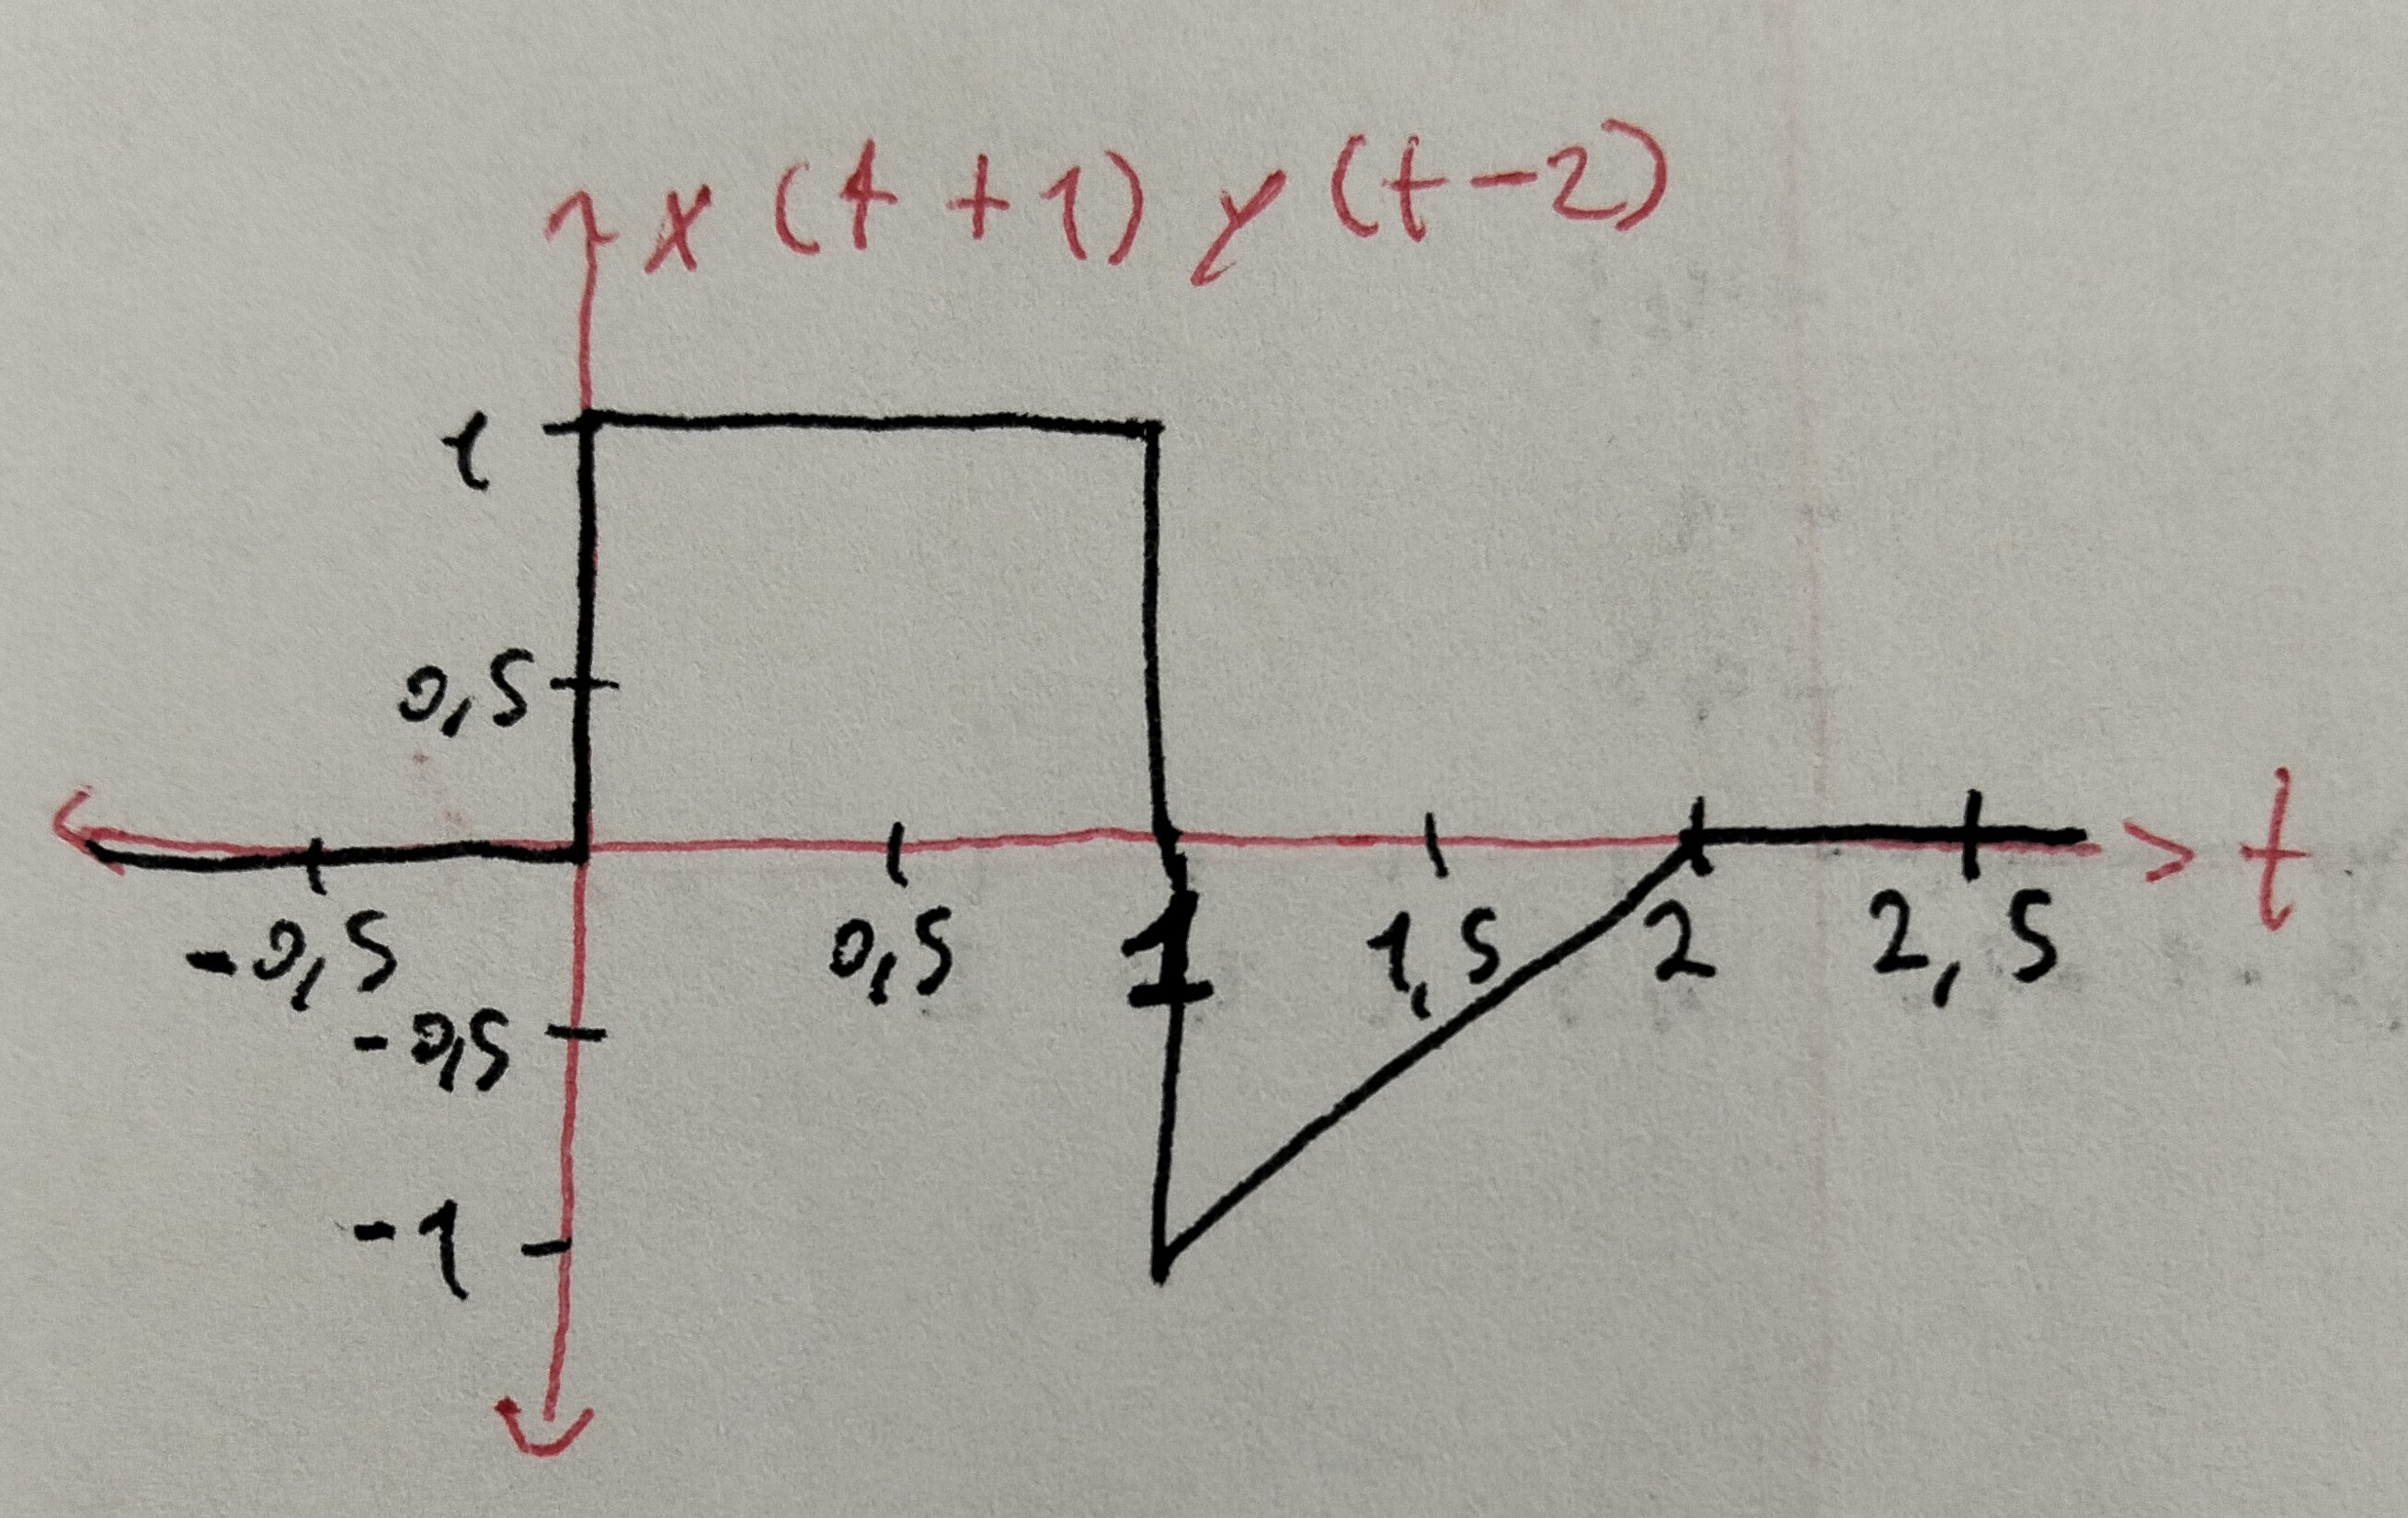
\includegraphics[width=0.6\textwidth]{Punto8Fig3.jpg}
    \caption{Señal $x(t+1)y(t-2)$}
\end{figure}

\textbf{d) Señal $x(t)y(-1-t)$}\\
El término $y(-1-t)$ es activo cuando $-1-t \in [-2, 2] \implies t \in [-3, 1]$. $x(t)$ es activa en $[-1, 3]$. Su área común es $t \in [-1, 1]$:
\begin{itemize}
    \item $t \in [-1, 0)$: $x(t) = -t-1$. El argumento de $y$ está en $(-1, 0]$, donde $y=-1$. Producto: $(-t-1)(-1) = t+1$.
    \item $t \in [0, 1]$: $x(t) = t$. El argumento de $y$ está en $[-2, -1]$, donde $y=1$. Producto: $(t)(1) = t$.
\end{itemize}

\begin{figure}[h!]
    \centering
    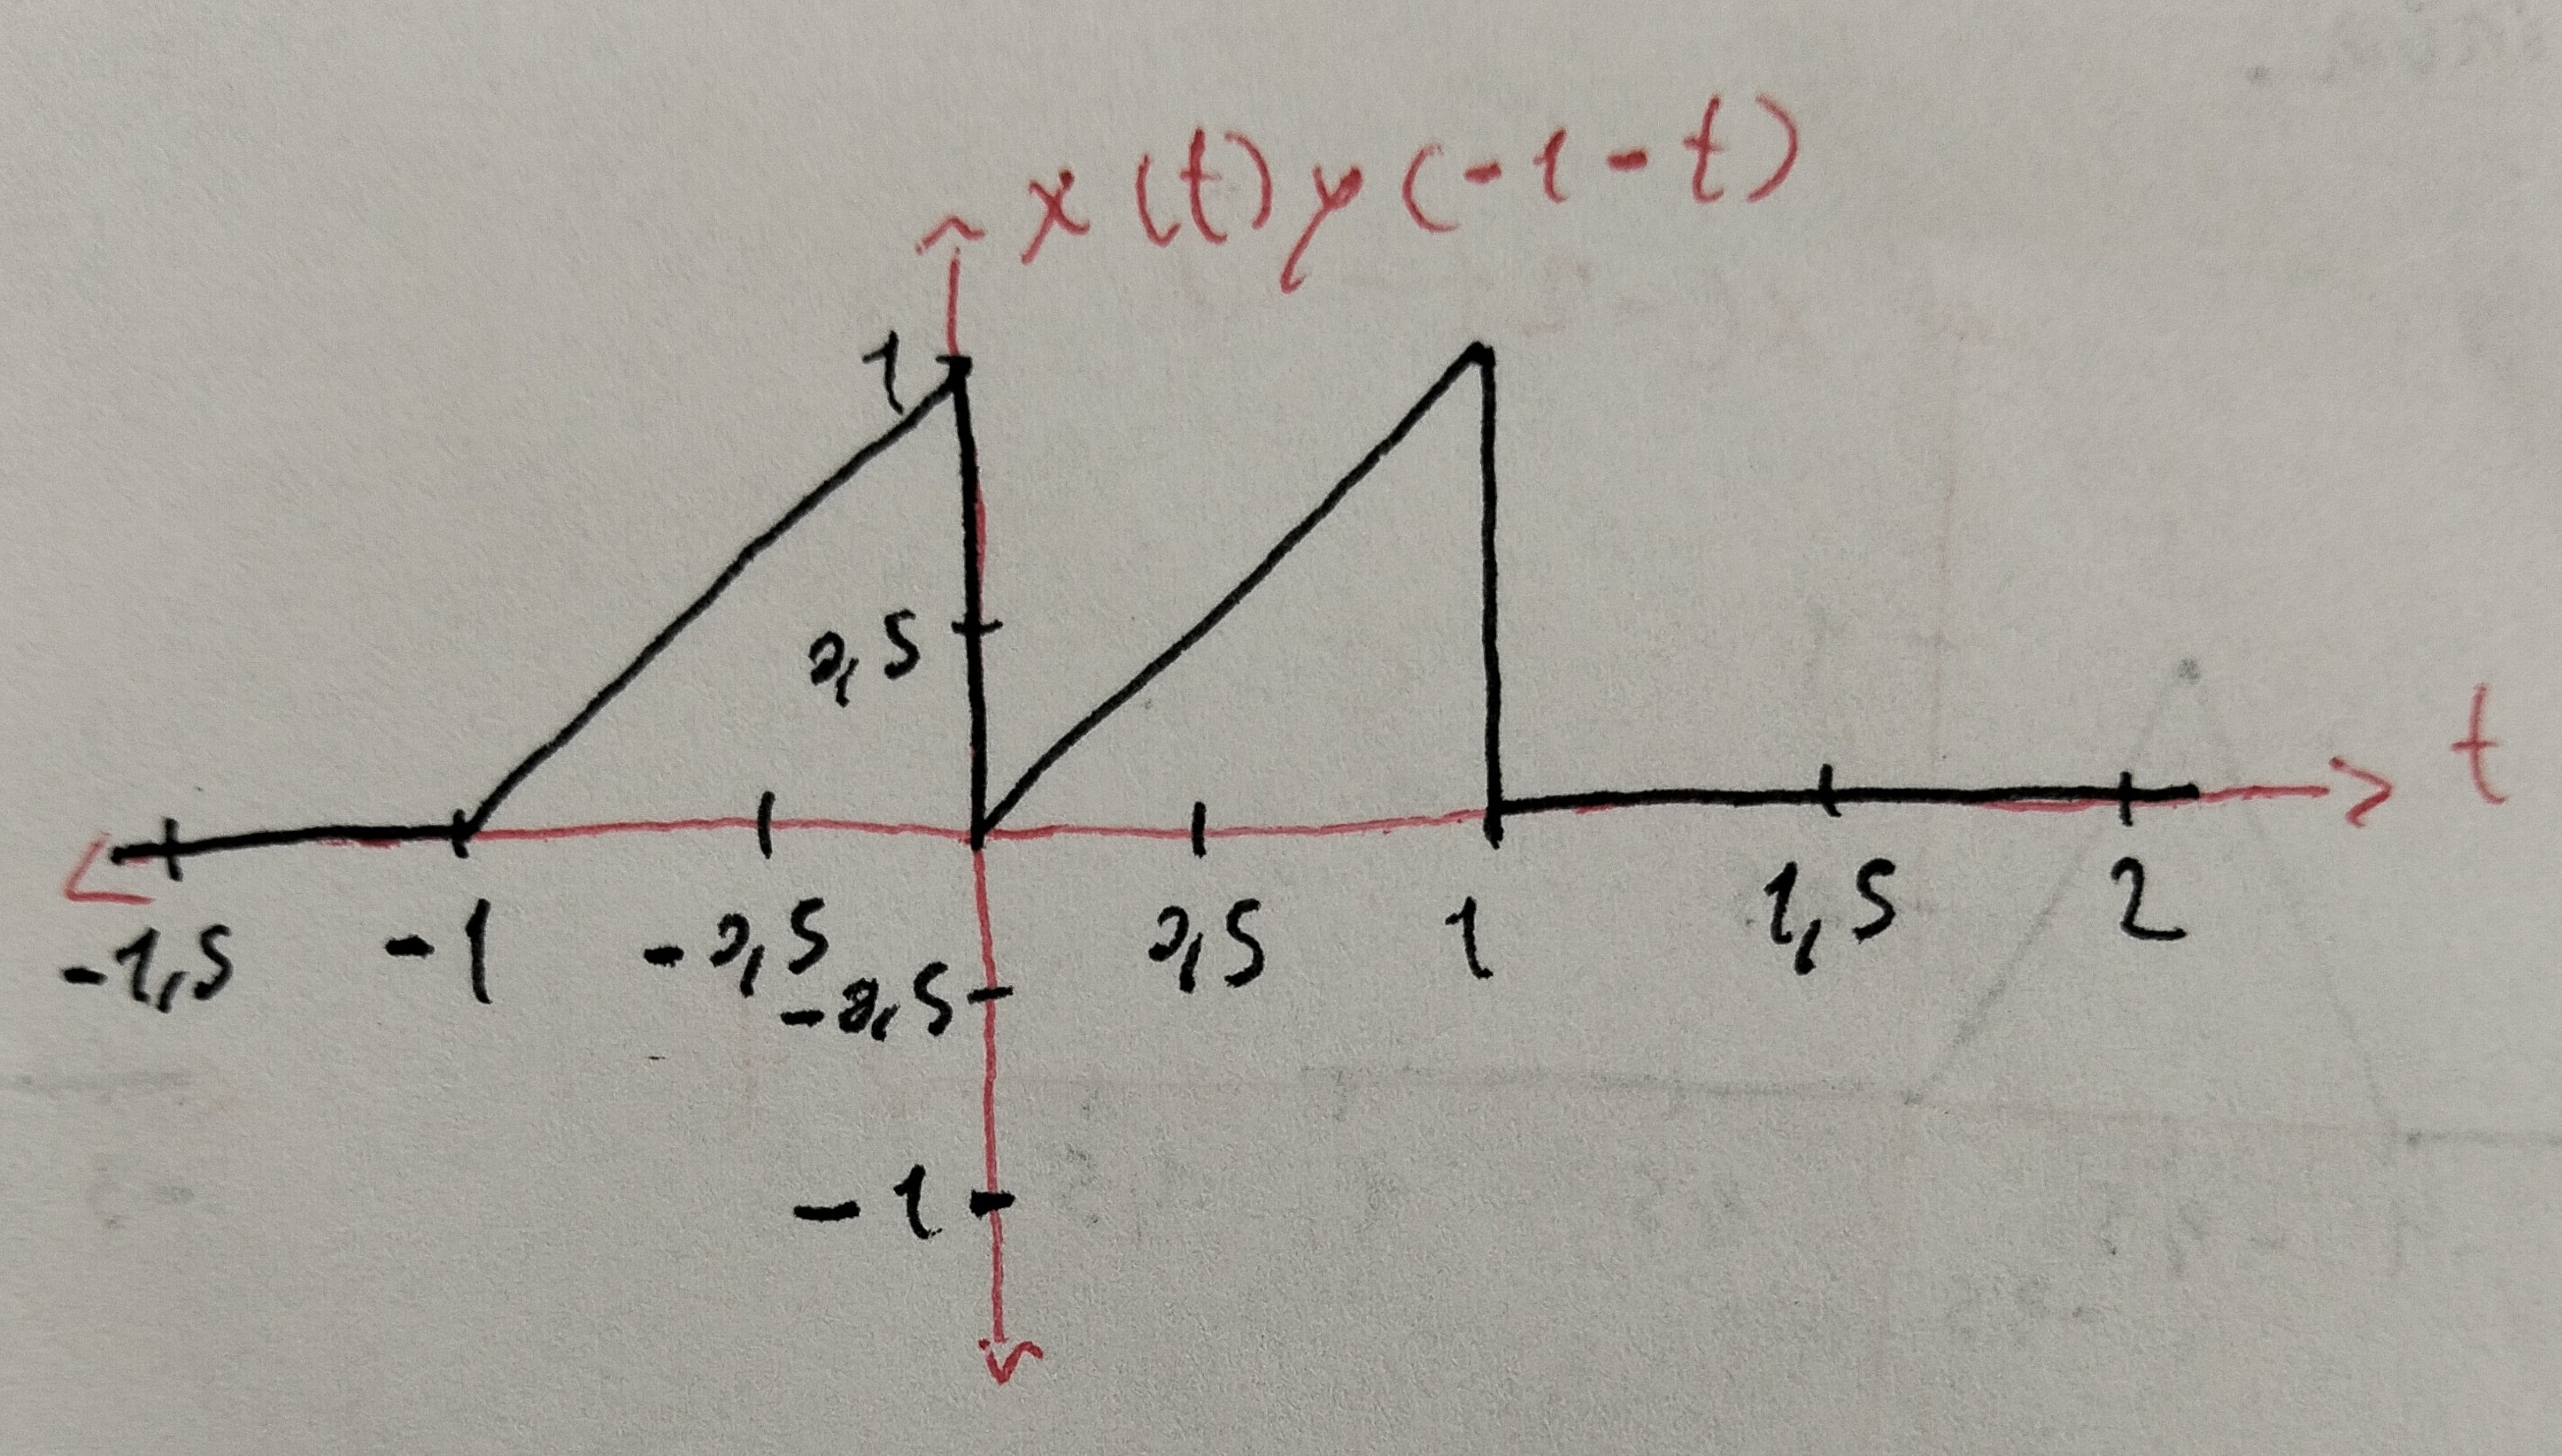
\includegraphics[width=0.6\textwidth]{Punto8Fig4.jpg}
    \caption{Señal $x(t)y(-1-t)$}
\end{figure}

\textbf{e) Señal $x(4-t)y(t)$}\\
El término $x(4-t)$ es no nulo cuando $4-t \in [-1, 3] \implies t \in [1, 5]$. Dado que $y(t)$ sólo es no nula en $[-2, 2]$, el único traslape ocurre en $t \in [1, 2]$.
\begin{itemize}
    \item Para $t \in [1, 2]$: el argumento $4-t$ pertenece a $[2, 3]$. Evaluando $x$ en este rango: $x(4-t) = 3 - (4-t) = t-1$.
    \item En este mismo rango, $y(t) = 1$. 
    \item El producto es $(t-1)(1) = t-1$.
\end{itemize}
La gráfica es cero en todo instante, excepto por una rampa lineal que asciende de $0$ a $1$ en el intervalo $t \in [1, 2]$.

\begin{figure}[h!]
    \centering
    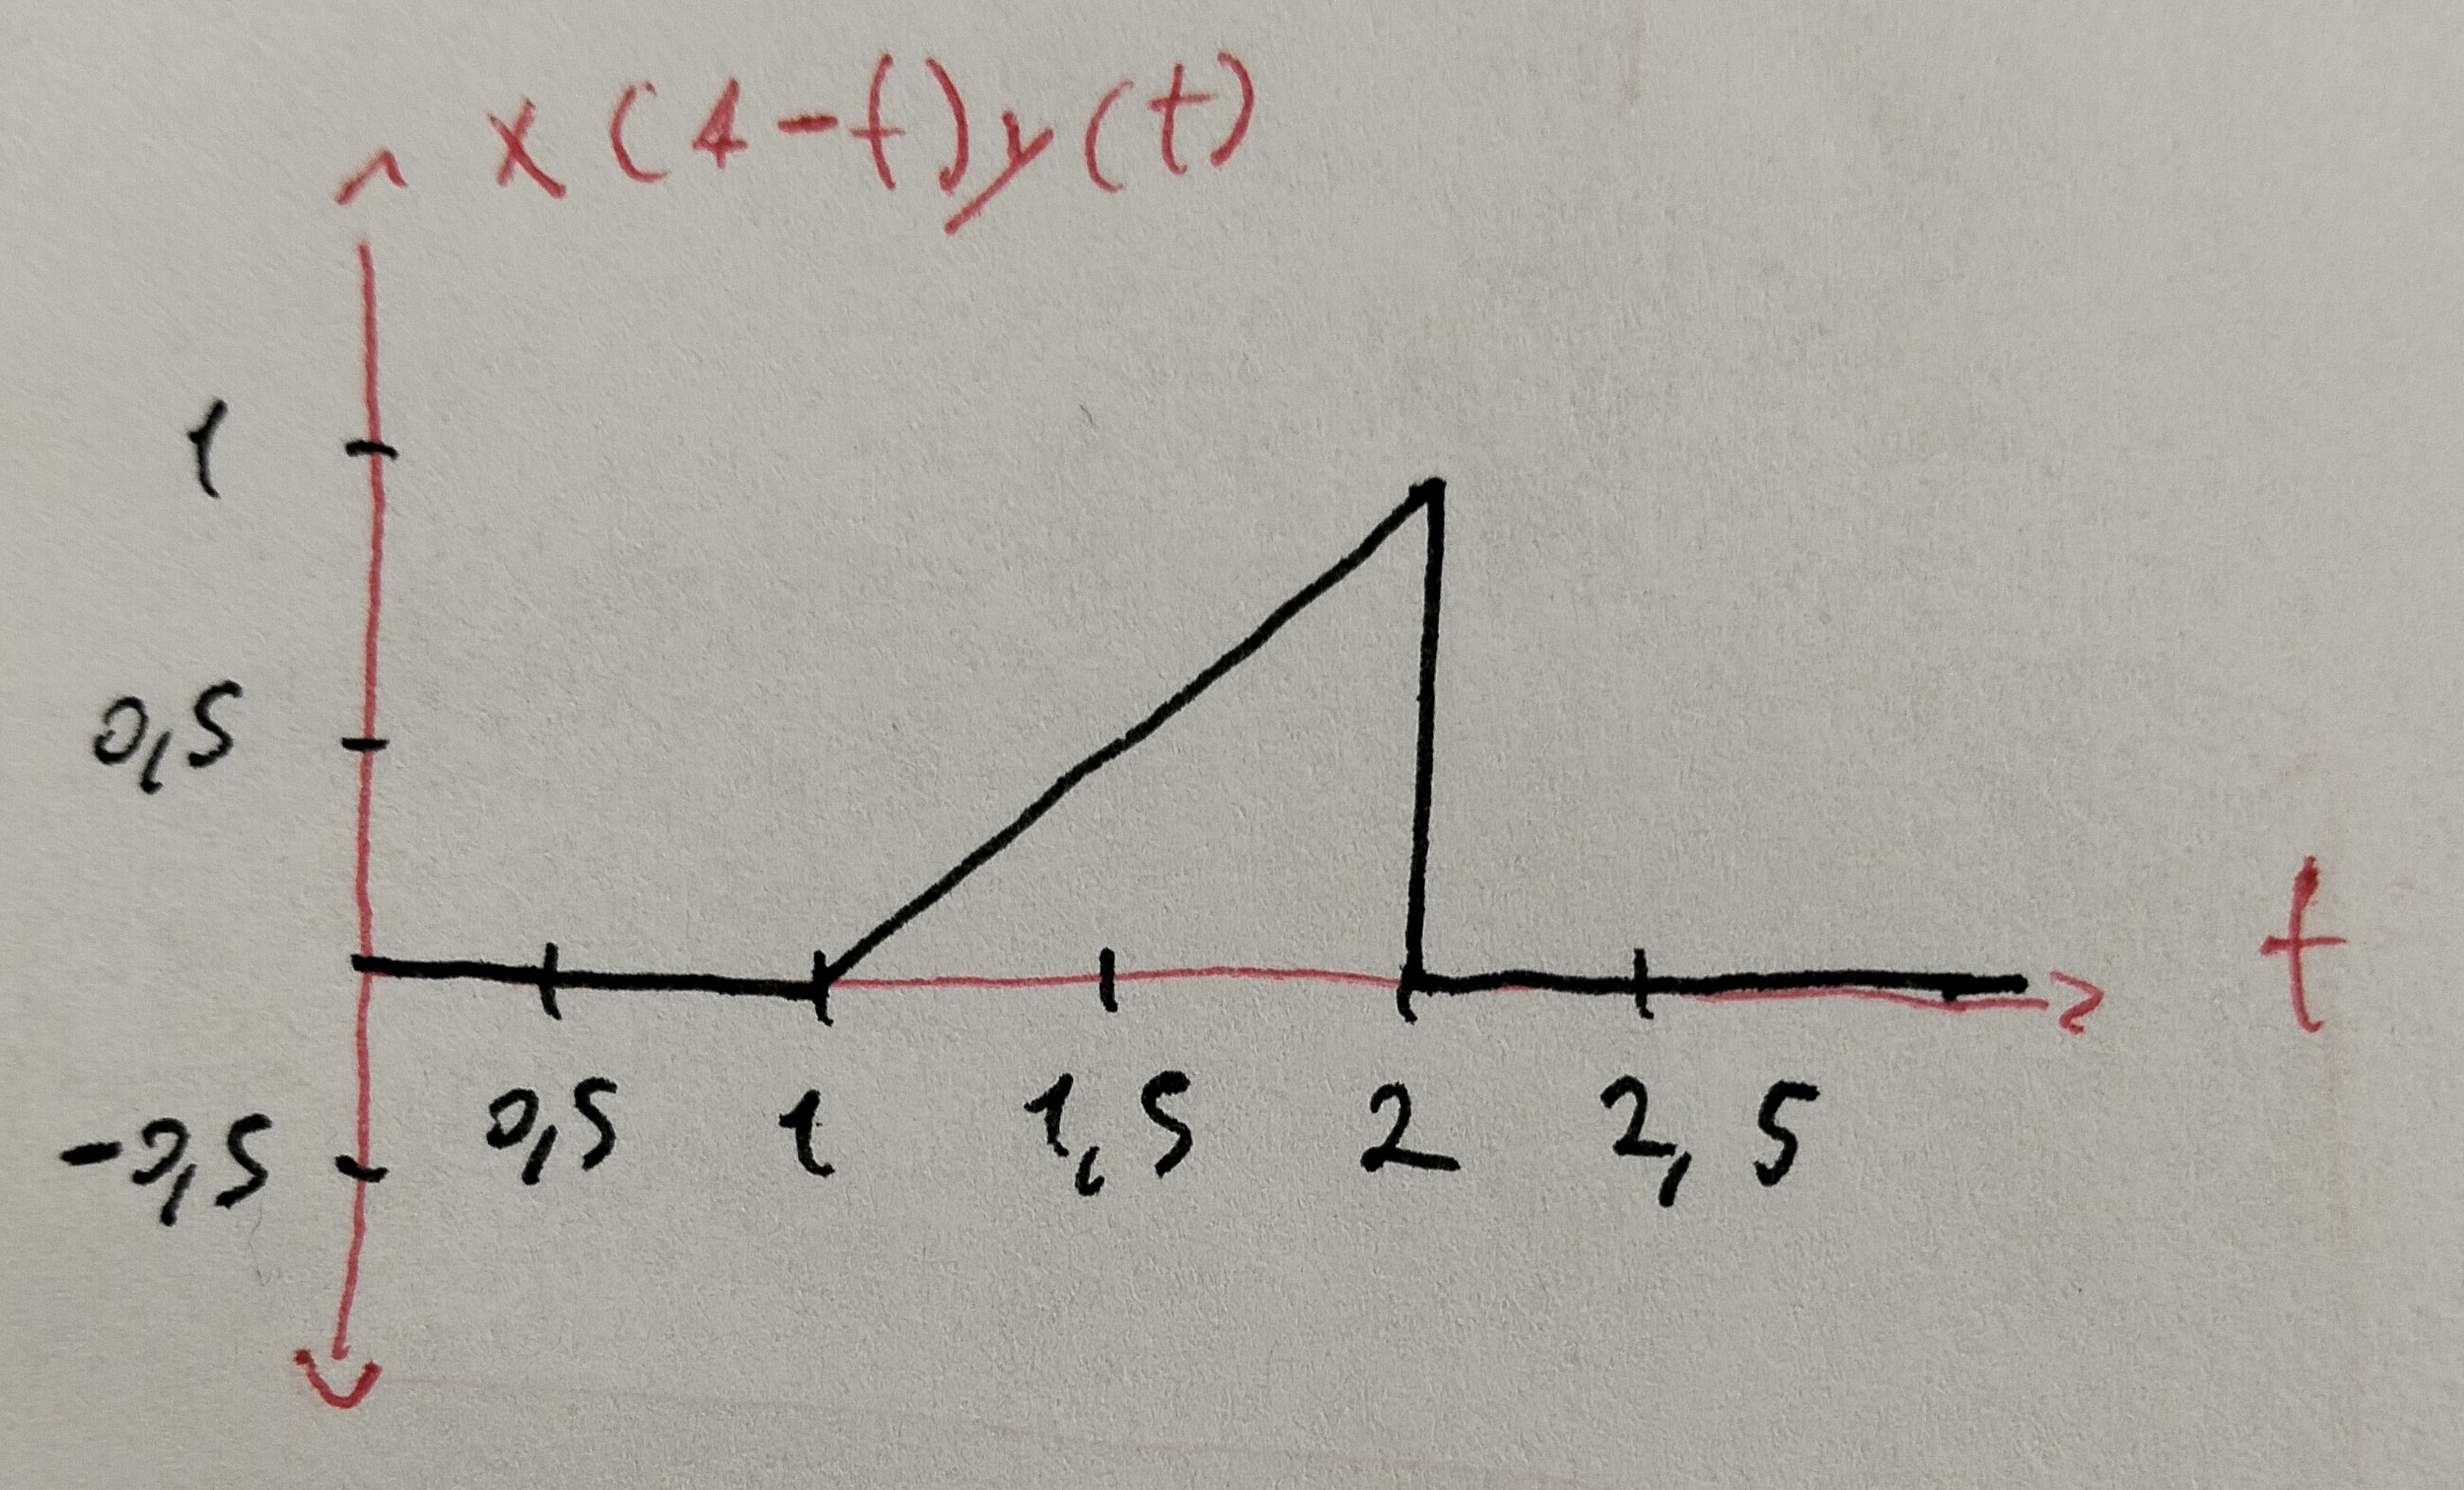
\includegraphics[width=0.6\textwidth]{Punto8Fig5.jpg}
    \caption{Señal $x(4-t)y(t)$}
\end{figure}

\subsection*{Solución del Punto 9: Dibujo de Señales}

Para graficar señales compuestas por funciones escalón unitario $\mu(t)$, debemos analizar los puntos de discontinuidad (donde cambian los argumentos) y evaluar la amplitud de la señal en cada intervalo de tiempo.

\subsubsection*{a) Primera Señal: $x(t) = \mu(t+1) - 2\mu(t) + \mu(t-1)$}

Los puntos críticos ocurren en $t = -1$, $t = 0$ y $t = 1$. Analizamos los tramos:
\begin{itemize}
    \item \textbf{Para $t < -1$:} Todos los escalones están apagados ($0$). 
    \[ x(t) = 0 - 0 + 0 = 0 \]
    \item \textbf{Para $-1 \leq t < 0$:} Solo se activa $\mu(t+1)$.
    \[ x(t) = 1 - 0 + 0 = 1 \]
    \item \textbf{Para $0 \leq t < 1$:} Se activan $\mu(t+1)$ y $\mu(t)$.
    \[ x(t) = 1 - 2(1) + 0 = -1 \]
    \item \textbf{Para $t \geq 1$:} Todos los escalones están activos.
    \[ x(t) = 1 - 2(1) + 1 = 0 \]
\end{itemize}

\textbf{Forma de la gráfica a mano:} Es un pulso rectangular que sube a $1$ en $t = -1$, cae abruptamente a $-1$ en $t = 0$, y vuelve a cero en $t = 1$.

\subsubsection*{b) Segunda Señal: $x(t) = -\mu(t+3) + 2\mu(t+1) - 2\mu(t-1) + \mu(t-3)$}

Los puntos críticos ocurren en $t = -3$, $t = -1$, $t = 1$ y $t = 3$. Evaluamos los tramos:
\begin{itemize}
    \item \textbf{Para $t < -3$:} Todo apagado. $\Rightarrow x(t) = 0$.
    \item \textbf{Para $-3 \leq t < -1$:} Se activa el primer escalón.
    \[ x(t) = -(1) + 0 - 0 + 0 = -1 \]
    \item \textbf{Para $-1 \leq t < 1$:} Se activa el segundo escalón.
    \[ x(t) = -1 + 2(1) - 0 + 0 = 1 \]
    \item \textbf{Para $1 \leq t < 3$:} Se activa el tercer escalón.
    \[ x(t) = -1 + 2 - 2(1) + 0 = -1 \]
    \item \textbf{Para $t \geq 3$:} Todos los escalones activos.
    \[ x(t) = -1 + 2 - 2 + 1 = 0 \]
\end{itemize}

\textbf{Forma de la gráfica a mano:} Comienza en cero, baja a $-1$ en $t = -3$, sube hasta $1$ en $t = -1$, vuelve a bajar a $-1$ en $t = 1$, y regresa finalmente a cero en $t = 3$.


\subsection*{Solución del Punto 10: Operaciones con Señales Discretas}

A partir de las gráficas dadas, extraemos los valores significativos de las señales base:
\[ x[n] = \{3_{n=-3}, 2_{n=-2}, 1_{n=-1}, 0_{n=0}, 1_{n=1}, 2_{n=2}, 3_{n=3}\} \]
\[ y[n] = \{-1_{n=-4}, -1_{n=-3}, -1_{n=-2}, -1_{n=-1}, 0_{n=0}, 1_{n=1}, 1_{n=2}, 1_{n=3}, 1_{n=4}\} \]

\subsubsection*{a) Primera Señal: $z_1[n] = x[n-2] + y[n+2]$}

Esta operación consiste en desplazar $x[n]$ hacia la derecha en 2 unidades, desplazar $y[n]$ hacia la izquierda en 2 unidades, y sumar sus amplitudes punto a punto:

\begin{itemize}
    \item \textbf{Para $n = -6$:} $x[-8] + y[-4] = 0 + (-1) = -1$
    \item \textbf{Para $n = -5$:} $x[-7] + y[-3] = 0 + (-1) = -1$
    \item \textbf{Para $n = -4$:} $x[-6] + y[-2] = 0 + (-1) = -1$
    \item \textbf{Para $n = -3$:} $x[-5] + y[-1] = 0 + (-1) = -1$
    \item \textbf{Para $n = -2$:} $x[-4] + y[0] = 0 + 0 = 0$
    \item \textbf{Para $n = -1$:} $x[-3] + y[1] = 3 + 1 = 4$
    \item \textbf{Para $n = 0$:} $x[-2] + y[2] = 2 + 1 = 3$
    \item \textbf{Para $n = 1$:} $x[-1] + y[3] = 1 + 1 = 2$
    \item \textbf{Para $n = 2$:} $x[0] + y[4] = 0 + 1 = 1$
    \item \textbf{Para $n = 3$:} $x[1] + y[5] = 1 + 0 = 1$
    \item \textbf{Para $n = 4$:} $x[2] + y[6] = 2 + 0 = 2$
    \item \textbf{Para $n = 5$:} $x[3] + y[7] = 3 + 0 = 3$
\end{itemize}
Cualquier otro valor de $n$ produce un resultado de $0$.

\subsubsection*{b) Segunda Señal: $z_2[n] = x[n+2] \cdot y[6-n]$}

Esta operación requiere multiplicar los valores de la señal desplazada a la izquierda $x[n+2]$ por la señal invertida y desplazada $y[6-n]$:

\begin{itemize}
    \item \textbf{Para $n = -5$:} $x[-3] \cdot y[11] = 3 \cdot 0 = 0$
    \item \textbf{Para $n = -4$:} $x[-2] \cdot y[10] = 2 \cdot 0 = 0$
    \item \textbf{Para $n = -3$:} $x[-1] \cdot y[9] = 1 \cdot 0 = 0$
    \item \textbf{Para $n = -2$:} $x[0] \cdot y[8] = 0 \cdot 0 = 0$
    \item \textbf{Para $n = 1$:} $x[3] \cdot y[5] = 3 \cdot 0 = 0$
\end{itemize}
Analizando los únicos instantes donde ambas señales tienen valores distintos de cero en simultáneo:
\begin{itemize}
    \item \textbf{Para $n = -1$:} $x[1] \cdot y[7] = 1 \cdot 0 = 0$
    \item \textbf{Para $n = 0$:} $x[2] \cdot y[6] = 2 \cdot 0 = 0$
\end{itemize}
Debido a que los intervalos donde las señales no son nulas no se cruzan tras las transformaciones temporales, el producto final de ambas señales es idénticamente nulo para todo valor de $n$:
\[ z_2[n] = 0, \quad \forall n \]


\subsection*{Solución del Punto 11: Periodicidad de Señales}

Para evaluar si una señal es periódica y encontrar su periodo fundamental, aplicamos las condiciones de periodicidad en tiempo discreto y continuo:

\subsubsection*{a) Primera Señal: $x[n] = \cos\left(\frac{8}{15}\pi n\right)$}

En tiempo discreto, una señal sinusoidal de la forma $x[n] = \cos(\omega_0 n)$ es periódica si y solo si la frecuencia angular $\omega_0$ dividido entre $2\pi$ es un número racional. 
Aquí, $\omega_0 = \frac{8}{15}\pi$. Evaluamos la relación:
\[ \frac{\omega_0}{2\pi} = \frac{\frac{8}{15}\pi}{2\pi} = \frac{8}{30} = \frac{4}{15} \]
Dado que $\frac{4}{15}$ es un número racional ($\mathbb{Q}$), la señal **es periódica**. El periodo fundamental en muestras, $N$, se calcula a partir de la fracción irreducible $\frac{m}{N} = \frac{4}{15}$ con $m=4$. Por lo tanto, el periodo fundamental es:
\[ N = 15 \text{ muestras} \]

\subsubsection*{b) Segunda Señal: $x(t) = \cos(2t) + \sin(3t)$}

En tiempo continuo, la suma de señales periódicas es periódica si la razón de sus periodos individuales es un número racional.
\begin{itemize}
    \item Para $\cos(2t)$: $\omega_1 = 2 \Rightarrow T_1 = \frac{2\pi}{2} = \pi$
    \item Para $\sin(3t)$: $\omega_2 = 3 \Rightarrow T_2 = \frac{2\pi}{3}$
\end{itemize}
Evaluamos la relación de periodos:
\[ \frac{T_1}{T_2} = \frac{\pi}{\frac{2\pi}{3}} = \frac{3}{2} \]
Como $\frac{3}{2}$ es racional, la señal **es periódica**. El periodo fundamental $T$ es el Mínimo Común Múltiplo (mcm) de los periodos o se obtiene cruzando la fracción ($T = 2T_1 = 3T_2$):
\[ T = 2(\pi) = 2\pi \text{ segundos} \]

\subsubsection*{c) Tercera Señal: $x[n] = \cos\left(\frac{1}{5}\pi n\right)\sin\left(\frac{1}{3}\pi n\right)$}

Utilizamos la identidad trigonométrica del producto de seno y coseno $\cos(A)\sin(B) = \frac{1}{2}[\sin(A+B) - \sin(A-B)]$ para descomponer la señal:
\[ x[n] = \frac{1}{2}\sin\left(\frac{8}{15}\pi n\right) - \frac{1}{2}\sin\left(-\frac{2}{15}\pi n\right) = \frac{1}{2}\sin\left(\frac{8}{15}\pi n\right) + \frac{1}{2}\sin\left(\frac{2}{15}\pi n\right) \]
Determinamos el periodo fundamental de cada componente analizando sus frecuencias angulares:
\begin{itemize}
    \item Componente 1: $\omega_1 = \frac{8}{15}\pi \Rightarrow \frac{\omega_1}{2\pi} = \frac{4}{15} \Rightarrow N_1 = 15$
    \item Componente 2: $\omega_2 = \frac{2}{15}\pi \Rightarrow \frac{\omega_2}{2\pi} = \frac{1}{15} \Rightarrow N_2 = 15$
\end{itemize}
El periodo fundamental general $N$ es el Mínimo Común Múltiplo (mcm) de $N_1$ y $N_2$:
\[ N = \text{mcm}(15, 15) = 15 \text{ muestras} \]

\subsection*{Solución del Punto 12: Impulso Aplicado a un Derivador}

Consideramos un pulso triangular simétrico $x(t)$ centrado en el origen, que va desde $t = -T/2$ hasta $t = T/2$, con altura $\frac{1}{2}T$ en la base (La amplitud de la forma de onda del pulso tiene un área igual a 1). La expresión formal de las pendientes del triángulo es:
\[ x(t) = \begin{cases} 
\frac{4}{T^2}t + \frac{2}{T}, & -\frac{T}{2} \leq t < 0 \\
-\frac{4}{T^2}t + \frac{2}{T}, & 0 \leq t \leq \frac{T}{2} \\
0, & \text{en otro caso}
\end{cases} \]

\subsubsection*{a) Salida $y(t)$ del derivador}

La salida de un sistema derivador es $y(t) = \frac{dx(t)}{dt}$. Derivando tramo por tramo la función lineal definida:
\[ y(t) = \begin{cases} 
\frac{4}{T^2}, & -\frac{T}{2} \leq t < 0 \\
-\frac{4}{T^2}, & 0 \leq t \leq \frac{T}{2} \\
0, & \text{en otro caso}
\end{cases} \]
Físicamente, la salida está constituida por dos pulsos rectangulares adyacentes de duración $T/2$: uno positivo de amplitud $\frac{4}{T^2}$ y uno negativo de amplitud $-\frac{4}{T^2}$.

\subsubsection*{b) Comportamiento cuando $T \to 0$}

Cuando el ancho del pulso $T$ tiende a cero, la amplitud $\frac{4}{T^2}$ tiende a infinito ($\infty$) y la duración tiende a cero de forma extremadamente rápida. Al aproximar las funciones en el límite empleando la distribución delta de Dirac $\delta(t)$, el pulso positivo se concentra en el lado izquierdo y el pulso negativo en el derecho. La combinación límite define formalmente al doblete unitario o la derivada de la delta de Dirac:
\[ \lim_{T \to 0} y(t) = \frac{d\delta(t)}{dt} = \delta'(t) \]

\subsubsection*{c) Área total bajo la salida $y(t)$}

Calculamos el área total integrando $y(t)$ en todo el dominio temporal:
\[ \text{Área} = \int_{-\infty}^{\infty} y(t) \, dt = \int_{-T/2}^{0} \frac{4}{T^2} \, dt + \int_{0}^{T/2} \left(-\frac{4}{T^2}\right) \, dt \]
\[ \text{Área} = \left[ \frac{4}{T^2}t \right]_{-T/2}^{0} + \left[ -\frac{4}{T^2}t \right]_{0}^{T/2} = \left(0 - \left(-\frac{2}{T}\right)\right) + \left(-\frac{2}{T} - 0\right) = \frac{2}{T} - \frac{2}{T} = 0 \]
El área total es **cero para cualquier valor de $T$**. Esto se justifica analíticamente porque el área del pulso positivo cancela de manera exacta el área del pulso negativo adyacente.

\subsubsection*{Conclusión: Resultado de derivar un impulso unitario}

Basado en las respuestas anteriores, la derivada de un impulso unitario $\delta(t)$ genera una función matemática singular llamada **doblete unitario** $\delta'(t)$. Esta señal se caracteriza por tener amplitudes infinitamente grandes y opuestas concentradas en $t=0$, con una duración nula y cuya área total neta bajo la curva es idénticamente cero.


\end{document}